\documentclass{cacthesis}

%Define your additional packages here
\usepackage{xcolor}
\usepackage{hyperref}
\usepackage{nameref}
\usepackage{tikz}
\usepackage{amsfonts}
\usepackage{amsthm}
\usepackage{macros}
\usepackage{capt-of}
\usepackage{dashbox}
\usepackage{diagbox}

\usepackage[
    backend=biber,
    style=alphabetic,
    %sortlocale=de_DE,
    %natbib=true,
    %url=false, 
    %doi=true,
    %eprint=false
]{biblatex}

\usepackage [
n, % or lambda
advantage , operators ,
sets ,
adversary , landau , probability , notions ,
logic ,
ff, mm,
primitives , events , complexity , oracles , asymptotics , keys
]{ cryptocode}

\addbibresource{references.bib}

\newcommand{\authnote}[3]{{ \footnotesize \textbf{#1[#2: #3]~}}}
\newcommand{\orfnote}[1]{\authnote{\color{blue}}{Orfeas}{#1}}
\newcommand{\niknote}[1]{\authnote{\color{red}}{Nikos}{#1}}

\newtheorem{definition}{Definition}

\begin{document}

	\frontmatter
	
	%%%%%%%%%%%%%
	%% Title page
	%%%%%%%%%%%%%
	\title{Trustless incoercible sale of physical goods over a blockchain}
	%\subtitle{Longer subtitle (if required)}	%Delete subtitle if not required
	\author{Nikolaos Stivaktakis}
	\date{September 26, 2019}
	\subject{Master Thesis}
	
	\publishers{
		\small
		\begin{tabular}{r l}
			Supervisors:  & Prof. Sebastian Faust, Ph.D. \\
			& 2nd supervisor \\
		\end{tabular}
	}
	\maketitle
	
	\section*{Abstract}
	Write an abstract
	
	\newpage
	
	%TODO Delete this comment for the final submission:
	\textcolor{red}{\textbf{!!! Prüfen Sie, dass der folgende Text aktuell ist (entsprechend der formalen Regeln des Studienbüros) !!! \\
	!!! Check that this text is up to date (according to formal rules of the examination office) !!!}}
	
	\section*{Erklärung zur Abschlussarbeit gemäß § 22 Abs. 7 APB TU Darmstadt}
	
	Hiermit versichere ich, \textcolor{red}{\textbf{Nikolaos Stivaktakis}}, die vorliegende Master-Thesis / Bachelor-Thesis gemäß § 22 Abs. 7 APB der TU Darmstadt ohne Hilfe Dritter und nur mit den angegebenen Quellen und Hilfsmitteln angefertigt zu haben. Alle Stellen, die Quellen entnommen wurden, sind als solche kenntlich gemacht worden. Diese Arbeit hat in gleicher oder ähnlicher Form noch keiner Prüfungsbehörde vorgelegen. 
	
	Mir ist bekannt, dass im Falle eines Plagiats (§38 Abs.2 APB) ein Täuschungsversuch vorliegt, der dazu führt, dass die Arbeit mit 5,0 bewertet und damit ein Prüfungsversuch verbraucht wird. Abschlussarbeiten dürfen nur einmal wiederholt werden.
	
	Bei einer Thesis des Fachbereichs Architektur entspricht die eingereichte elektronische Fassung dem vorgestellten Modell und den vorgelegten Plänen.
	
	\vspace{10pt}
	\hrule
	
	\section*{English translation for information purposes only:\\Thesis Statement pursuant to § 22 paragraph 7 of APB TU Darmstadt}
	
	I herewith formally declare that I, \textcolor{red}{\textbf{Nikolaos Stivaktakis}}, have written the submitted thesis independently pursuant to § 22 paragraph 7 of APB TU Darmstadt. I did not use any outside support except for the quoted literature and other sources mentioned in the paper. I clearly marked and separately listed all of the literature and all of the other sources which I employed when producing this academic work, either literally or in content. This thesis has not been handed in or published before in the same or similar form.
	
	I am aware, that in case of an attempt at deception based on plagiarism (§38 Abs. 2 APB), the thesis would be graded with 5,0 and counted as one failed examination attempt. The thesis may only be repeated once.
	
	For a thesis of the Department of Architecture, the submitted electronic version corresponds to the presented model and the submitted architectural plans.
	
	\vspace{10pt}
	\hrule
	\vspace{70pt}
	
	\noindent\begin{tabular}{l@{\hskip 1in}l}
		\makebox[1.8in]{\hrulefill} & \makebox[3.5in]{\hrulefill}\\
		Datum / Date & Unterschrift / Signature
	\end{tabular}
	
	\listoffigures
	\listoftables
	\tableofcontents
	
	\mainmatter
	
	\chapter{Introduction}
	\niknote{Say in a trade without trust: who sends first? which is a big part of the dilemma.}
The remote and anonymous nature of blockchains greatly complicates the sale of physical goods over a blockchain: Since the item is physical and therefore unknown to the blockchain, one cannot build a smart contract that atomically exchanges it for its price. In addition to that, the anonymity of both the seller and the buyer make it virtually impossible to build a robust recovery mechanism if one party pays/sends honestly first but the other misbehaves afterwards.
The most common solution is to add a trusted third party which obtains both the coins and the good before sending them to their recipients. As third parties can misbehave and there are scenarios where no trusted third party is available, a protocol that is not relying on a trusted third party is beneficial.\newline

The goal of this thesis is to examine whether such a protocol can exist. For that, we first have to formalize the problem. We have to define the requirements for such a protocol, what properties such a protocol has to meet in order to realize a trustless and incoercible sale. We take a game-theoretic approach to model the behaviour of the different parties: Each party is modeled rational, meaning that each party is trying to maximize its own utility/payoff/profit? We want to find a protocol where it is profitable for each party to not deviate from this protocol. If such a protocol is found, as it is in the best interest of the parties to follow the protocol, it solves the problem of a sale without trust. The seller can expect the Buyer to pay not because of trust, but because it is the most profitable option for the buyer himself. We propose various candidates and analyse if these proposed protocols do indeed meet the criteria to be such a protocol. \newline

%\niknote{the text from the mail}
%The goal of this project is to answer this question positively. We propose a scheme in which the parties lock on-chain some collateral which will only be released if they agree on-chain on the success or failure of the sale, otherwise burnt. To avoid coercion, after sending the payment the buyer ignores messages from the seller, on receipt of the item asks a trusted (only by the buyer) party to verify whether the item is the expected good or not and reports the answer to the blockchain. If, before paying, the buyer can credibly threaten the seller that she will stick to this strategy after paying, then it is, we believe, provable that coercion is impossible. A number of ideas to achieve such a credible threat while minimizing the needed trust exist

	\section{Motivation}
	%why is it worth to write my master thesis about this topic?
	%Whats the big picture? How is this master thesis contributing to this big picture?
	
	%\subsection{why}
	%why physical good? what is the difference to digital goods? Why we are looking at selling\newline
	%
	In the last years there has been a big rise of the digital world and cryptocurrencies. As they gain acceptance, they become a valid payment option for sales of digital and physical goods. Current solutions work with a trusted third party, an escrow, that collects the payment and the good and then forward them to their recipients. In order for this solution to work, both parties have to trust the third party. There exist situations where there is no trusted third party and these solutions are not viable. Worse, if the two parties trust a third party that is not trustworthy, there is a possibility that they lose all the money that is involved in this trade. \niknote{maybe mention the big amount of scams in the ctypto world} Therefore there is a demand for trustless solutions which solve the problem without needing a trusted third party. \newline
	
	While a trustless sale of digital goods over the blockchain is possible and there are existing solutions \cite{asgaonkar_solving_2019}, the sale of physical goods are much more complicated as the good and its delivery are unknown to the blockchain. Finding a protocol that enables a trustless and incoercible sale of physical goods over a blockchain would make cryotocurrencies more useful as a currency and allow potential sellers to sell physical goods directy to their clients without any risk involved.\newline 
	
	%a sale Many economic processes are based on trust. .. because of the rise of the digital world and the irregulated nature of cryptocurrencies, economic parties often can not trust the other parties: A Buyer does not trust a unknown Seller without any reputation and vice-versa (look at the many scams in the crypto market) . That is the reason why there is a need for protocols that work with a minimal amount of trust.
	%\subsection{what}
	%to find a protocol that enables a sale of a physical good over a blockchain: The payment of the price occurs over a blockchain. This sale has to be trustless (no trusted third party) and incoercible (One party can not coerce the other party into doing something they do not want)
	
	%What we need: Blockchain, Smart Contract
	%We look at the problem with 2 players: One Seller one Buyer
	%emphasise that normally this is done with a trusted third party, but we want to find a protocol with NO trusted third party.
	%\subsection{how}
	%same problem, different solution proposals easiest solution, then more complex per iteration until we find solution that works as simple as possible, as complex as necessary say	collateral? that we did one side collateral then both side collateral (and did the protocols that make the most sense). and each with 3 versions: first sellere, first buyer, both simultaneous)
   %% we assumed, if it is possible, a possible protocol would be found by us in this step.
    %First search the most probable solutions, after finding out that they do not work, try to proof that it is impossible with this set of assumptions, therefore ease up the assumptions and propose new solution.
	\section{Methodology}
	We take an iterative approach to find a solution to our problem. We first propose the simplest possible solution and analyse if it indeed solves our problem. If yes, we are finished. If no, we add a layer of complexity and propose a new solution. This cycle will be continued until we find a solution or we think we exhausted the most probable solutions and there is no solution to the proposed problem. If this is the case we try and proof that there is no solution to the proposed problem.
	%With this approach we try to find a solution as simple as possible but as complex as necessary.
	\section{Structure of this thesis}
	In chapter 2 preliminaries, 3 related work...
\section{Related work}
\minisec{\citetitle{asgaonkar_solving_2019}\cite{asgaonkar_solving_2019}}
In this paper \citeauthor{asgaonkar_solving_2019} proposed a protocol that allows the sale of a digital good without a trusted third party. Their solution involves a Smart Contract that collects a deposit from both the selling and the buying party. If then one party misbehaves, the Smart Contract slashes the deposit of the lying party.  This solution assumes the good to be digitally verifiable. Therefore if one party is not honest, the opposing honest party can report this misbehaviour to the Smart Contract and proof that the other party indeed did misbehave. The authors also provide a game-theoretic analysis of their protocol and confirm that honest behaviour is the only Nash equilibrium.

\minisec{\citetitle{zimbeck_two_nodate}\cite{zimbeck_two_nodate}}
In this work \citeauthor{zimbeck_two_nodate} proposes a protocol based on bitcoin scripts that should allow the trade between two perfect strangers even if the parties themselves can not be trusted. His approach has no need for a trusted third party. \citeauthor{zimbeck_two_nodate} also implemented his protocol in an open source program called BitHalo. His approach was formally and game-theoretically analysed in the paper \cite{bodei_validation_2015}

\minisec{\citetitle{kiayias_escrow_2017}\cite{kiayias_escrow_2017}}
In this paper \citeauthor{kiayias_escrow_2017} look at the problem of buying physical goods using cryptocurrencies with a third party acting as an escrow. They formalized the escrow problem for physical goods and introduce multiple schemes with different properties. 
\chapter{Preliminaries}
\section{Game Theory}
\niknote{first generaly describe the field}
Game theory studies the interaction between self-interested players \cite{leyton-brown_essentials_2008}. It uses models to analyse games.
\niknote{a little bit of history}
It is considered that the field began in 1944 with the publication of von Nemann \& Morgenstern's "The Theory of Games and Economic Behaviour" \cite{rasmusen_games_nodate,vonNeumannTheory} Then Nash... history   What is a game?? Each player wants to \cite{leyton-brown_essentials_2008-1} 
%As discribed in \cite{kiayias_escrow_2017}, 
\subsection{Games}
A game consists of players who are taking actions in order to maximize their own payoff. An action is a choice that a player can make. Each possible action for a given decision is contained in an action set. Which choice the player makes is influencing how big his payoff will be. The payoff (or utility) is a numerical value and each player gets his own payoff.
\begin{definition}[Game]
A game is a tuple ($N$,$A$,$u$), where:
\begin{itemize}
    \item $N$ is a finite set of n players
    \item $A = A_1 \times \dots \times A_n$, where $A_i$ is a finite set of actions available to player i. Each vector $a= (a_1,...,a_n) \in A$ is called an action profile.
    \item $u_1,...,u_n$ where $u_i$: $A \to \mathbb{R}$ is a payout (or utility) function for player i.
\end{itemize} {\normalfont \cite{leyton-brown_essentials_2008}}
\end{definition}
\subsection{Strategies}
Each player faces multiple decisions in a game. At every decision point he chooses between possible actions. These decision can depend on every information that the player knows at this stage of the game. Which action a player takes in which situation can be formulated in a strategy. A possible strategy could be: If the opposing player takes action $L$, I will take action $R$, else i will take action $L$.
\begin{definition}
Player $i$'s strategy $s_i$ is a rule that tells him which action to choose at each instant of the game, given his information set. {\normalfont \cite{rasmusen_games_nodate}}.
\end{definition}
We call the set of every strategy for a player his strategy set. A strategy profile is an ordered set consisting of one strategy for each of the n players in the game.
- best response
-dominated and dominant strategies here
\subsection{Nash Equilibrium}
tell something about nash\newline
what about pareto/strictly dominated strategies equilibrium?
\begin{definition}[Nash Equilibrium]
A strategy profile $s^*$ is a Nash equilibrium if no player has incentive to deviate from his strategy given that the other players do not deviate. {\normalfont \cite{rasmusen_games_nodate}} Formally: \[\forall i: \forall s_i': u(s^*_i,s^*_{-i}) \geq u(s'_i,s^*_{-i})\].
\end{definition}
strict/weak nash
\subsection{Turn-based games}
\begin{definition}[turn-based games]
\label{def:turn-based-game}
A game is turn-based if only one party can play at a time and its move is revealed
to all other parties before the next move.
\end{definition}
To analyse turn-based games we will use game trees. The nodes of the tree represent decision points and the edges of the tree possible actions. The leafs of the tree are the payout values for the players. In this example Alice and Bob have one decision each. Alice will play first. She has the possible actions $L$ and $R$. Then Bob will make his decision choosing between the actions $L$ and $R$. \newline

\orfnote{Game trees and
examples should be introduced in the preliminaries. Mention that, in our work, a
game is turn-based if only one party can play at a time and its move is revealed
to all other parties before the next move. Mention that we can combine
simultaneous and turn-based games if some moves are turn-based and some are
simultaneous.}


\orfnote{for the example, prefer parties $A$, $B$ instead
of $B$, $S$. For actions, you can e.g. use $L$, $R$, which is common in Game
Theory literature for generic moves when every choice is binary. Do not use the
same payouts everywhere. Better use specific numbers. Use numbers with a single
Nash Equilibrium and walk the reader through the analysis of why it is a Nash
Equilibrium.}


\begin{figure}[htb!]
\begin{tikzpicture}[sibling distance=7cm,level distance=6em,every node/.style={shape=circle,align=center}]
      \node[draw]{$A$}
        child{node[draw]{$B$}
                child[sibling distance = 3cm]{node[shape = rectangle]{$1_A|6_B$} edge from parent node [left] {$L$}} 
                child[sibling distance = 3cm]{node[shape=rectangle]{$5_A | 5_B$}edge from parent node [right] {$R$}} edge from parent node [left] {$L$}} 
        child{node[draw]{$B$}
            child[sibling distance = 3cm]{node[shape=rectangle]{$4_A | 2_B$}edge from parent node [left] {$L$}}
            child[sibling distance = 3cm]{node[shape = rectangle]{$3_A | 3_B$}edge from parent node [right] {$R$}}edge from parent node [right] {$R$}};
\end{tikzpicture}
    \centering
    \caption{Example Tree}
    \label{fig:example-tree}
\end{figure}

To find the Nash Equilibrium of this game we will use the method "iterated elimination of strictly dominated strategies".
\niknote{TODO look for paper,  more information here}\newline

To analyze the game we start at the bottom of the tree at Bob's decision. He always takes the action that yields him the biggest payout.  We start at the left branch. If Bob takes action $L$, he gets a payout of $6$. If he chooses action $R$, he gets a payout of $5$. In this scenario Bob chooses $L$, because $6>5$.
On the right branch he chooses $R$ because $3>2$.\newline

Then we look at Alice's decision. She knows that Bob chooses the path that yields him the greatest payout and can calculate his decisions. She knows that Bob will choose $L$,if Alice takes action $L$. Therefore her payout of action $L$ is $1$. If she chooses action $R$, Bob will choose $R$ as well. In this case Alice has a payoff of $3$. Alice chooses action $L$, because $3>1$.\newline

The Nash Equilibrium of this game is \{$R$,$R$\} and the payout is $3_A | 3_B$.
\subsection{Simultaneous games}
\begin{definition}[Simultaneous games]
\label{def:simultaneous-game}
A game is simultaneous, if at least two parties play at a time. 
\end{definition}

To analyse simultaneous games we will use a table. The two players are again Alice and Bob. On the top of the table we see the possible strategies of Bob: \emph{be honest} and \emph{lie}. On the left side are the possible strategies for Alice: \emph{report} and \emph{hide}. For each combination of strategies the two parties get a specific payout. For example if Bob chooses strategy \emph{lie} and Alice chooses strategy hide, Bob gets a payout of 8 and Alice gets a payout of 2.

\begin{table}[htb!]
    \centering
    \begin{tabular}{ |c||c|c| }
    \hline
    \diagbox{\color{red}Alice}{\color{blue}Bob}& \emph{be honest} & \emph{lie}  \\
    \hline
    \hline
    \emph{report} & {\color{red}$2$} $|$ {\color{blue}$5$} & {\color{red}$5$} $|$ {\color{blue}$-3$} \\
    \hline
    \emph{hide} & {\color{red}$2$} $|$ {\color{blue}$3$} & {\color{red}$2$} $|$ {\color{blue}$8$} \\
    \hline
    \end{tabular}
    \caption{Example Table}
    \label{tab:example-table}
\end{table}

If we now look at the table we can see which combinations of strategy benefits which player. There is a Nash Equilibrium at \{\emph{be honest}, \emph{report}\}, because no player can improve their payout by changing strategy. If bob changes his his strategy to \emph{lie}, his payout will decrease to $-3$. If a Alice changes her strategy to \emph{hide}, she will get the exact same payout of 2. Because Alice's payout does not decrease, this Nash Equilibrium is a weak Nash Equilibrium.

\section{Cryptographic primitives}

\niknote{do i need a general introduction to the field of cryptography?}
\section{Public Key Cryptography}
\niknote{We use some PK cryptography, maybe I should explain it a little to the reader}
\subsection{Commitment schemes}
Commitment schemes are used in a vast variety of cryptographic protocols. They enable a party to commit itself to a value while keeping it secret \cite{Goldreich2001-bv}. This resembles a non transparent sealed envelope: By putting a note in such an envelope, a party commits itself to the content of the note. This note can not be read until the envelope is being opened.  \niknote{maybe delete}\newline 

 A commitment scheme lets one party (Bob) commit to a value of his choice. Later, he can open the commitment in order to convince another party (Alice) that indeed that value was committed. Committing to a value results in a commitment string $c$, that Bob sends to Alice, and an opening string $s$ that Bob uses for opening the commitment later\cite{boneh_graduate_nodate}.\newline
 
 A commitment scheme is secure if it satisfies the following two properties:
 \begin{itemize}
     \item \textbf{Hiding:} The Commitment string $c$ reveals no information about the commited value\cite{boneh_graduate_nodate}.
     \item \textbf{Binding:} Let $c$ be a commitment string output that Bob gets by committing the value $v$. Bob can open this commitment to the committed value $v$, but not to any other value $v'\neq v$.
 \end{itemize}
 %Bob shares the commitment string with Alice. In a later stage Bob can open the committment using the co ommitment schemes have two algorithms: \emph{Commit} and \emph{Open}. In the committing phase a party can use \emph{commit} to turn a value into a commitment and an opening value. In addition to the commitment the algorithm also returns an opening value. Later, the commitment can be "opened" with that exact opening value. and it returns a value. The returned value is guaranteed to be the value to which the party committed in the committing phase. If any party\cite{Goldreich2001-bv}. 
\section{Cryptocurrencies}
\niknote{look at that again}
Cryptocurrencies are decentralised currencies that introduce a way to transfer value with low latency and without any intermediary. They use various cryptographic primitives to prevent fraud. An important cryptographic tool are digital signatures, that ensure that only the owner of the coin can spend it. Hash algorithms allow For this work, it is not important to understand these cryptographic primitives. A detailed description of said crypgtographic primitives can be found at Katz and Lindell's book \emph{Introduction into modern Cryptography} \cite{Katz2020-aj}. 

We will explain some of the principles of cryptocurrencies by looking at The first and best known cryptocurrency: Bitcoin. Bitcoin was introduced in 2008 Satoshi Nakamoto \cite{nakamoto_bitcoin_nodate}. In Bitcoin everyone can create his own wallet and send and receive coins. These coins are sent using transactions. Every transaction is stored on a public database, the blockchain (c.f. section~\ref{sec:blockchain}). Once these transactions are on the blockchain, they can never be changed or deleted. The blockchain acts as a public ledger recording all the transactions. The blockchain is maintained by the miners \niknote{what is a miner? how deep should I explain? as miners do not have something to do with my thesis directly} \newline

After Bitcoin many other cryptocurrencies were developed. In this work, we do not look at a specific cryptocurrency. We rather use them as a remote way to transfer value between two parties. These two parties do not need to know each other, rather they only need each other's wallet address to send coins to each other. The transfer of value occurs nearly instantaneous and can not be reversed.
\subsection{Blockchain}
\label{sec:blockchain}
In this work we look at public blockchains used for cryptocurrencies. In this context a blockchain is a public, distributed database storing every transaction. These transactions are grouped in blocks, where every block is linked with the previous block, forming a chain of blocks. \niknote{maybe a figure explains it best}   New transactions are written to the blockchain in the form of new blocks that are appended to the blockchain. As new transactions are posted constantly, the blockchain is always growing. This property is called \emph{liveliness}. Another important property is that blockchains are \emph{immutable}, which means whatever is written on the blockchain can not be altered.

properties: immutability, liveliness 

Cryptography is being used to secure these properties
Digital Signatures:\cite{Katz2020-aj} 
talk mostly about its properties
\subsection{Smart Contracts}

\chapter{Formalization}
% Example usage of definition START
%begin{definition}[Darmstadt]
%\label{def:darmstadt}
%Colon city
%\end{definition}
%Definition~\ref{def:darmstadt} transliterates Darmstadt.
% Example usage of definition END

\begin{definition}[Utility Function]
\label{def:utility-function}
The utility function $U_P(G)$ describes how much utility a physical good $G$ provides to a player $P$. The output of this function is a numerical value, which corresponds to the amount of coins that have equal value as $U_P(G)$. In this work, utility will always be a positive integer.
\end{definition}

\section{Entities}

\begin{definition}[Seller]
\label{def:seller}
A rational entity $S$ that owns a specific physical good $G$. The seller
has bigger utility in owning $P$ coins in contrast to owning $G$ (c.f.~equation~\ref{eq:seller-utility}) He therefore desires to exchange $G$ against $P$ coins.
\end{definition}

%Insert Utility function distribution
\begin{equation}
\label{eq:seller-utility}
    U_S(G) + P > P > U_S(G) > 0
\end{equation}

\begin{definition}[Buyer]
\label{def:buyer}
A rational entity $B$ that owns at least $P$ coins. The Buyer has greater utility in owning $G$ in contrast to  owning $P$ coins (c.f.~equation~\ref{eq:buyer-utility}). He therefore desires to exchange $P$ coins against $G$.
\end{definition}

%Insert Utility function distribution
\begin{equation}
\label{eq:buyer-utility}
    U_B(G) + P > U_B(G) > P > 0
\end{equation}

\orfnote{The SC is not really an escrow, as it doesn't hold on to the physical
good, only the money}
\orfnote{This definition is not detailed enough. You may introduce the exact
SC code here (discussing collateral/handling of $P$ in case of
disagreement as well), or at least refer to it TODO: rethink code location}
\niknote{I am a little unsure, how I want to define SC}
\begin{definition}[Smart Contract]
An entity SC that should ensure that the trade is successful. It acts as a fully trusted oracle.
\end{definition}

\section{The Game} \niknote{is this the right headline??}
\label{sec:the-game}
\begin{definition}[Initial State]
\label{def:initial-state}

\niknote{look at that definition again}
A Seller and a Buyer have some way of communicating with each other. A successful trade is beneficial for both entities. Both parties have enough funds in the given cryptocurrency to carry out protocol actions. The Seller is in possession of the physical good.
\end{definition} 


\begin{definition}[Desired Final State]
\label{def:desired-final-state}
The Buyer is in possession of the physical good and his funds have decreased by amount $P$. The funds of the seller have increased by $P$.
\end{definition}

\begin{definition}[Success of the trade]
The trade is considered successful if the situation transitions from the Initial State to the Desired Final State.
\end{definition}

We make the following assumptions:
\begin{enumerate}
    \item All entities have access to the Smart Contract and know the addresses and public keys of each other.
    \label{ass:1}
    \item The seller knows the physical address to which the buyer wants the good to be shipped. This address is not necessarily the buyer's real physical address, he can choose any physical address he wants to protect his privacy.
    \label{ass:2}
    \item Other than the information of assumption \ref{ass:1} and \ref{ass:2}, the buyer and the seller know nothing about each other.
    \label{ass:3}
    \item Both parties can send funds in the given cryptocurrency to any address.
    \label{ass:4}
    \item The sender has the power to send/ship the physical good to any physical address he wants.
    \label{ass:5}
    \item Both the seller and the buyer know the code of the Smart Contract.
    \label{ass:6}
    \item The seller and the buyer behave rationally, meaning that they both want to maximise their expected payout.
    \item Both $U_S(G)$ and $U_B(G)$ are positive. 
\end{enumerate}

We do not analyse transaction fees. 

\subsection{Goal}
\label{sec:goal}
The goal of this work is to design a protocol in which behaviour that results in a successful trade is a Nash Equilibrium. Minimal trust should be required. This will be achieved, if it is the rational behaviour for both players to perform the trade. A successful trade should be a Nash Equilibrium: If the other party behaves honestly, the best strategy will be to behave honestly as well.\niknote{Repitition? redundant?}\newline

%If the other party behaves rational it should be best to behave honest.
Another goal is that the trade is incoercible against rational attacks. That means that it should be unprofitable attack and decrease the payout of the other player, if the other player is honest. If this goal is achieved, a it is unprofitable, a rational Player will never try and attack the opposing player. It should be noted that that an irrational player can attack the opposing party, as an attack is unprofitable, but not necessarily impossible. If a player is willing to lower his own utility, he can attack an opposing honest player. 

\orfnote{The "Success of the trade" seems a bit too mixed with the "goal". Try
to express it in a clear way, maybe even merging the two concepts.}
\niknote{now okay? I set success of the trade as a pure definition. Goal is in text form and describes a little more}

%\subsection{Implementation}
%The underlying blockchain is immutable as long as there is an honest majority of %miners. We assume this honest majority.

\chapter{Candidate Two-Party Protocols}
In this chapter we try to find a two-party protocol that solves the proposed problem. We start by a simple, naive approach and then increase the complexity on each proposed protocol. On each protocol we examine the created game and analyze the Nash Equilibrium of that game. As described in section~\ref{sec:the-game}, we want to create a game where the Nash Equilibrium lies in an honest trade between the Seller and the Buyer.

\section{First try: no collateral}
\label{sec:first-try-nocol}
The simplest protocol is both players sending their resources without any collateral nor a third party. In this case there are 3 possibilities:
\begin{figure}[htb!]
\fbox{
 \procedureblock[linenumbering]{Buyer sends first}{
    \text{Buyer sends $P$ coins to the Seller}\\
    \text{Seller sends the physical good $G$ to the Buyer}
}
}
    \centering
    \caption{Protocol: No collateral, Buyer sends first}
    \label{pro:naive-buyer-first}
\end{figure}

\begin{figure}[htb!]
\fbox{
 \procedureblock[linenumbering]{Seller sends first}{
    \text{Seller sends the physical good $G$ to the Buyer}\\
        \text{Buyer sends $P$ coins to the Seller}
}
}
    \centering
    \caption{Protocol: No collateral, Seller sends first}
    \label{pro:naive-seller-first}
\end{figure}

\begin{figure}[htb!]
\fbox{
 \procedureblock[linenumbering]{Both players send simultaneously}{
    \text{Buyer sends $P$ coins to the Seller and seller sends $G$ to the Buyer simultaneously}}
}
    \centering
    \caption{Protocol: No collateral, both players send at simultaneously}
    \label{pro:naive-simultaneous}
\end{figure}

%Here maybe a visualization

\subsection{Possible strategies}
\label{sec:possible-strategies}
There is a countless amount of possible strategies for the two players. For example, a player can follow the protocol and trade honestly, he can try and gain an advantage by not following the protocol, he can ignore all messages or he can send all his money to the other party. It is not sensible to list and analyse all the possible strategies. We will concentrate on the strategies where a player follows the protocol and the strategies where a player intentionally deviates from the protocol to gain an advantage. As soon as we find a strategy for a player that is more profitable than following the protocol, we know that this protocol is not achieving our goals, as a rational player will not follow it. If we conclude that following the protocol is the most profitable strategy for both players, we know that this protocol is achieving our goal. \niknote{look at the end of this paragraph again} \newline

For the protocols proposed in section~\ref{sec:first-try-nocol} we analyse two strategies for each player. The Buyer can choose between strategy \emph{Pay} where he behaves honestly and sends the money and strategy \emph{Withhold} where the Buyer behaves dishonestly and does not send the money. The Seller can choose as well between strategy \emph{Send} where he sends the good $G$ and strategy \emph{Keep} where the Buyer does not send the $G$.
\subsection{Game: The Buyer acts first}
\begin{figure}[htb!]
\begin{tikzpicture}[sibling distance=7cm,level distance=6em,every node/.style={shape=circle,align=center}]
      \node[draw]{$B$}
        child{node[draw]{$S$}
                child[sibling distance = 7cm]{node[shape = rectangle]{$P-U_S(G)|U_B(G)-P$} edge from parent node [left] {\emph{Send}}} 
                child[sibling distance = 7cm]{node[shape=rectangle]{$P|-P$}edge from parent node [right] {\emph{Keep}}} edge from parent node [left] {\emph{Pay}}} 
        child{node{0$|$0} edge from parent node [right] {\emph{Withhold}}};
\end{tikzpicture}
\centering
\caption{No collateral, Buyer acts first}
\label{fig:nocol-buyer-first}
\end{figure}
%\captionof{figure}{Naive approach, Buyer sends first}

To analyze the game, we use the method "iterated elimination of strictly dominated strategies"\niknote{refer to preliminaries/source}. We start at the bottom at the seller's decision.
\begin{itemize}
    \item The Seller chooses \emph{Keep} (Because $P > P - U_S(G)$).\niknote{Do you like this format with itemize? I want the decisions to visually stand out}
\end{itemize}
    We then go one step towards the root and look at the Buyer's decision. He already knows that if he chooses \emph{Pay}, the rational Seller will choose \emph{Keep}. This would leave the Buyer with a payout of $-P$. If the Buyer chooses \emph{Withhold}, his payout is $0$.
\begin{itemize}
    \item The Buyer chooses \emph{Withhold} (Because $0 > -P$)
\end{itemize} 
%Therefore the Buyer has to choose between a payout of 0 (by choosing \emph{Withhold}) and $-P$ (by choosing \emph{Pay}). Since $0 > -P$, he chooses \emph{Withhold}.\newline
The Nash Equilibrium of this game is \{\emph{Keep}, \emph{Withhold}\} and results in a payout of $0|0$. Both parties are not sending anything and the trade is unsuccessful.

\subsection{Game: The Seller acts first} 

\begin{figure}[htb!]
\begin{tikzpicture}[sibling distance=7cm,level distance=6em,every node/.style={shape=circle,align=center}]
      \node[draw]{$S$}
        child{node[draw]{$B$}
                child[sibling distance = 7cm]{node[shape = rectangle]{$P-U_S(G)|U_B(G)-P$} edge from parent node [left] {\emph{Pay}}} 
                child[sibling distance = 7cm]{node[shape=rectangle]{$-U_S(G)|U_B(G)$}edge from parent node [right] {\emph{Withhold}}} edge from parent node [left] {\emph{Send}}} 
        child{node{0$|$0} edge from parent node [right] {\emph{Keep}}};
\end{tikzpicture}
\centering
\label{fig:nocol-seller-first}
\caption{No collateral, Seller acts first}
\end{figure}


The analysis is similar to the above case, but the roles are reversed. 
\begin{itemize}
    \item The Buyer would choose \emph{Withhold} as $U_B(G) > U_B(G)-P$
    \item The seller would choose \emph{Keep} as $0 > -U_S(G)$
\end{itemize}
The Nash Equilibrium of this game is \{\emph{Keep}, \emph{Withhold}\} and results in a payout of $0|0$. Again, both parties are not sending anything and the trade is unsuccessful.

\subsection{Game: Both parties act simultaneously} 

\begin{table}[htb!]
    \centering
    \begin{tabular}{ c||c|c| }
    & \emph{Pay} & \emph{Withhold}  \\
    \hline
    \hline
    \emph{Send} & $P - U_S(G)|U_B(G) - P$ & $-U_S(G) | U_B(G)$ \\
    \hline
    \emph{Keep} & $P |-P$ & $0 | 0$ \\ 
    \hline
    \end{tabular}
    \label{fig:nocol-simultaneous}
    \caption{No collateral: Both parties send simultaneously}
\end{table}
If we look at the payout table we can see that \emph{Withhold} dominates \emph{Pay} and \emph{Keep} dominates \emph{Send}. These strategies provide a bigger payout regardless of the strategy of the other party.
Since we assume the players to be rational, they would both choose the dominant strategy.
Again, the Nash Equilibrium of this game is \{\emph{Keep}, \emph{Withhold}\} and results in a payout of $0|0$. As the Nash Equilibrium does not correspond to the Desired Final State (c.f.~Definition \ref{def:desired-final-state}), this game does not satisfy our goal.\newline

It is interesting to note that this table resembles the famous prisoner's dilemma, where the Nash Equilibrium is not Pareto efficient. We can see that \{\emph{Keep}, \emph{Withhold}\} is not the Pareto optimal case, because \{\emph{Send}, $Pay\}$ increases the payout of both parties. 
In other words, a successful trade would benefit both parties but is not happening in this game as it is not the Nash Equilibrium. \niknote{last sentence redundant?}
%TODO explain Prisoners dilemma? Pareto Efficient
%The Nash Equilibrium is on both parties not sending anything, still both parties would yield a bigger payout if they just traded successfully. 


%\section{Second Try: One-Sided collateral}  \orfnote{apply earlier notes that also suit here}

\section{Second Try: Buyer Collateral}
\label{sec:buyer-collateral}
To incentivize an entity to follow the protocol we introduce collateral. The collateral will be lost if the entity deviates from the protocol. In this section we will look at a protocol where only one the Buyer deposits collateral. We introduce a Smart Contract~(SC) which handles the collateral. The payment $P$ is now routed via the Smart Contract.  \newline

Following protocol is proposed:
\begin{figure}[htb!]
\fbox{
 \procedureblock[linenumbering]{Buyer Collateral protocol}{
     \text{Buyer deposits collateral $C > P$ to the Smart Contract}\\
    \text{Seller sends the physical good $G$ to the seller}\\
    \text{After receiving $G$, the Buyer sends funds of amount $P$ to the Smart Contract}\\
    \text{The Smart Contract releases the collateral of the Buyer and sends $P$ to the Seller}
}
}
    \centering
    \caption{Buyer Collateral protocol}
    \label{pro:buyer-col}
\end{figure}

The Smart Contract releases the collateral as soon as it receives $P$ by the Buyer. By paying $P$, the Buyer implicitly reports to the Smart Contract that he has received the physical good $G$. The collateral should incentivize the Buyer to pay the Seller after receiving the physical good $G$, as his collateral is greater than $P$.\newline

It is important that the Seller sends first, as he has no collateral and therefore no incentive to follow the protocol. If we swap the order and let the Buyer send first, the Seller will simply keep $G$ and be in possession of both $G$ and $P$. Because of the collateral, the Seller can safely send $G$ first without having to worry that the Buyer will not pay him.\newline

\subsection{Possible Strategies}
\label{sec:possible-strategies-buyercol}
We still have the strategies from section~\ref{sec:possible-strategies}: \emph{Pay} and \emph{Withhold} for the Buyer and \emph{Keep} and \emph{Send} for the Seller. The The Buyer now has one additional decision: He can either follow the protocol and deposit the collateral $C$ (\emph{Deposit}) or deviate from the protocol and refuse to deposit the collateral (\emph{Refuse}).

\subsection{Game}
\begin{figure}[htb!]
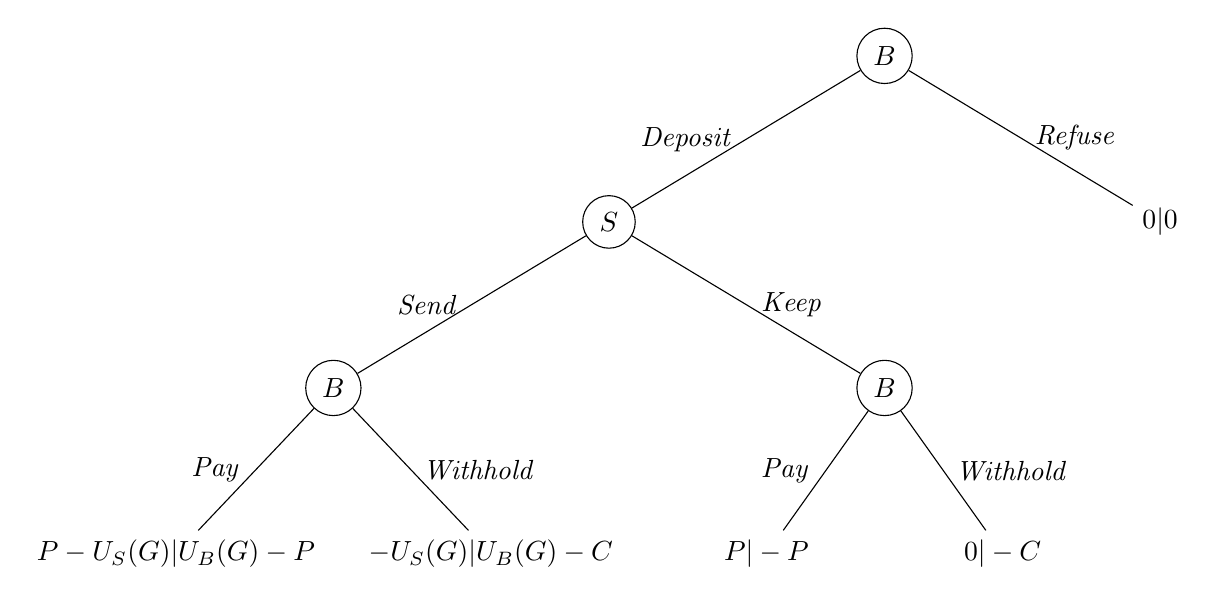
\begin{tikzpicture}[sibling distance=7cm,level distance=6em,every node/.style={shape=circle,align=center}]
      \node[draw]{$B$}
        child{node[draw]{$S$}
                child[sibling distance = 7cm]{node[draw]{$B$}
                		child[sibling distance = 4cm]{node[shape = rectangle]{$P-U_S(G)|U_B(G)-P$} edge from parent node [left] {\emph{Pay}}} 
                		child[sibling distance = 4cm]{node[shape=rectangle]{$-U_S(G)|U_B(G)-C$}edge from parent node [right] {\emph{Withhold}}} edge from parent node [left] {\emph{Send}}} 
                child[sibling distance = 7cm]{node[draw]{$B$}
                child[sibling distance = 3cm]{node[shape = rectangle]{$P|-P$} edge from parent node [left] {\emph{Pay}}} 
                child[sibling distance = 3cm]{node[shape=rectangle]{$0|-C$}edge from parent node [right] {\emph{Withhold}}}edge from parent node [right] {\emph{Keep}}} edge from parent node [left] {\emph{Deposit}}} 
          child[sibling distance = 7cm]{node[shape = rectangle]{$0|0$}edge from parent node [right]{\emph{Refuse}}};
\end{tikzpicture}
\centering
    \caption{Only the Buyer deposits collateral}
\end{figure}
To analyze the payout of this game, we again start at the bottom at the Buyer's decision. On both branches the Buyer chooses \emph{Pay}:
\begin{itemize}
    \item $U_B(G) - P > U_B(G) - C$
    \item $-P > -C$
\end{itemize}
We now look at the Seller's decision. He chooses \emph{Keep}:
\begin{itemize}
    \item $P > P-U_S(G)$
\end{itemize}
This means that it is better for the Seller to behave maliciously and not send the physical good $G$. The Buyer would send $P$ just to get back his collateral but receive nothing more, leaving him with a payout of $-P$. At the root of the tree the Buyer chooses $Refuse$:
\begin{itemize}
    \item $-P < 0$
\end{itemize}
The Nash Equilibrium is at \{\emph{Refuse}\} and results in a payout of $0|0$. The trade is unsuccessful. \newpage


\section{Third Try: Seller Collateral}
\label{sec:seller-col}
In this section we will look into protocols where only the Seller deposits collateral.\newline

Following protocol is proposed:
\begin{figure}[htb!]
\fbox{
 \procedureblock[linenumbering]{Seller collateral protocol}{
    \text{Seller deposits collateral $C > P$ to the Smart Contract}\\
    \text{Buyer sends funds of amount $P$ to the seller}\\
    \text{Seller sends the physical good to the Buyer}\\
    \text{Buyer receives the physical good and confirms it to the Smart Contract}\\
    \text{The Smart Contract releases the collateral of the Seller}
}
}
    \centering
    \caption{Seller collateral protocol}
    \label{pro:seller-col}
\end{figure}

The collateral should incentivize the Seller to behave honestly and to ship the
physical good to the buyer. The Buyer can report to the SC with a simple boolean input:
\begin{itemize}
    \item 0 denotes that $G$ was not received
    \item 1 denotes that $G$ was received
\end{itemize}
%Because of the collateral, behaving honestly should be the best strategy for the seller.
\subsection{Possible Strategies}
\label{sec:possible-strategies-sellercol}
There are still the basic strategies from section~\ref{sec:possible-strategies}: \emph{Pay} and \emph{Withhold} for the Buyer and \emph{Keep} and \emph{Send} for the Seller. Similar to the strategies of the Buyer Collateral protocol (c.f.~\ref{sec:possible-strategies-buyercol}) the Seller has the option to deposit the collateral (\emph{Deposit}) or refuse to deposit the collateral (\emph{Refuse}).\newline

The Buyer has a unique opportunity: He decides what happens to the Seller's
collateral as he can either report that he received the physical good $G$ (\emph{Report}) or he can report that he did not receive it. Because he has this power over the Seller's collateral, he can try and coerce the Seller into sending him extra resources. This
strategy will be denoted as \emph{Coerce}.  After receiving the physical good he communicates to the Seller: "I will only report that I received the good if you send me back my payment $P$". It is important to see that this is a credible threat, because the Buyer's payout is not affected by him reporting or not reporting. Still,he has to find a way to convince the Seller that this statement is true. For the coercion to work, the Seller has to be convinced that he will indeed receive back his collateral if he sends the Payment $P$ back to the Seller. One possible way of convincing the Seller is via a second Smart Contract set up by the Buyer. As soon as the payment $P$ is sent back to the Buyer, this second SC will automatically report 1 to the first Smart Contract and the Seller's collateral is released. If the Buyer chooses \emph{Coerce}, the Seller
has two possible actions: He can comply and send back $P$ (\emph{Comply}) or not comply
and ignore the message (\emph{Ignore}).\newline

\subsection{Game}
\begin{figure}[htb!]
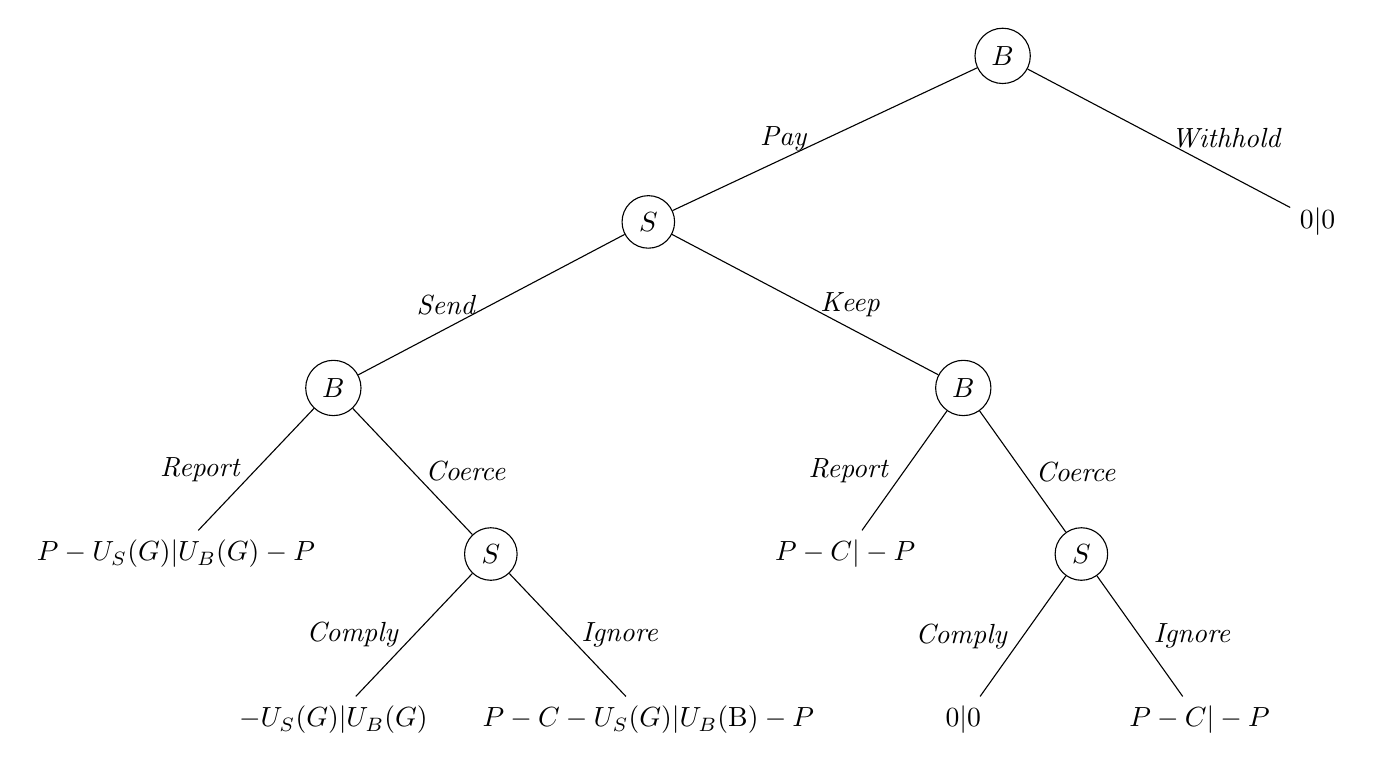
\begin{tikzpicture}[sibling distance=7cm,level distance=6em,every node/.style={shape=circle,align=center}]
      \node[draw]{$B$}
        child[sibling distance = 9cm]{node[draw]{$S$}
                child[sibling distance = 8cm]{node[draw]{$B$}
                		child[sibling distance = 4cm]{node[shape = rectangle]{$P-U_S(G)|U_B(G)-P$} edge from parent node [left] {\emph{Report}}} 
                		child[sibling distance = 4cm]{node[draw]{$S$}
                		    child[sibling distance = 4cm]{node[shape=rectangle]{$-U_S(G)|U_B(G)$} edge from parent node [left] {\emph{Comply}}}
                		    child[sibling distance = 4cm]{node[shape=rectangle]{$P-C-U_S(G)|U_B($B$)-P$} edge from parent node [right] {\emph{Ignore}}}edge from parent node [right] {\emph{Coerce}}} edge from parent node [left] {\emph{Send}}} 
                child[sibling distance = 8cm]{node[draw]{$B$}
                    child[sibling distance = 3cm]{node[shape = rectangle]{$P-C|-P$} edge from parent node [left] {\emph{Report}}} 
                    child[sibling distance = 3cm]{node[draw]{$S$}
                        child[sibling distance = 3cm]{node[shape=rectangle]{0$|$0} edge from parent node [left] {\emph{Comply}}}
                        child[sibling distance = 3cm]{node[shape=rectangle]{$P-C|-P$} edge from parent node [right] {\emph{Ignore}}}edge from parent node [right] {\emph{Coerce}}}edge from parent node [right] {\emph{Keep}}} edge from parent node [left] {\emph{Pay}}} 
          child[sibling distance = 8cm]{node[shape = rectangle]{$0|0$}edge from parent node [right] {\emph{Withhold}}};
          \centering
\end{tikzpicture}
\caption{Only the Seller deposits collateral}
\end{figure}

To analyze the payout, we again start at the bottom. Since $C>P$, The Seller would choose \emph{Comply} on both instances:
\begin{itemize}
    \item $-U_S(G) > P-C-U_S(G)$
    \item $0 > P-C$
\end{itemize}
One step above, the Buyer chooses \emph{Coerce} on both instances:
\begin{itemize}
    \item $U_B(G)> U_B(G)-P$
    \item $0 > -P$
\end{itemize}
Based on this information the Seller chooses \emph{Keep}: 
\begin{itemize}
    \item $0> -U_S(G)$
\end{itemize}
That means that both options for the Buyer would result in a payout of $0|0$. It does not matter which option he chooses.
The Nash Equilibrium is at \{Withhold\} \niknote{am I describing the Nash Equilibria correctly?} and results again at a payout of $0|0$.  The trade not successful.
%If $B$ sends the coins (does not choose strategy \emph{Withhold}), $S$ has to make the following decision: Does he send the good (\emph{Send}) or not (\emph{Keep})? We have to take into account, that $B$ decides what happens with the collateral. \newline
%If $S$ does not behave honestly (does not send the good), $B$ can punish $S$ by reporting 0 to the Smart contract. This means, that the collateral would not be given back to $S$.
What was designed to be an incentive for $S$ to behave honestly, ended up as leverage for $B$ over $S$. $B$ can report 0 (and burn the collateral) even if $S$ behaves honestly. 
%Therefore $B$ can use this leverage to coerce $S$ into giving him extra resources: “Give me C/2 coins or I will report 0 to the Smart Contract and burn your collateral.“
%Since sending the good has no impact on the collateral (the rational buyer will always play strategy $C_B$ over \emph{Pay}), it is best for $S$ to not send the physical good (\emph{Withhold}).
%Because not Sending (\emph{Keep}) is the best strategy for the seller, it is best for $B$ to not even send P and therefore not engage in the trade at all (\emph{Withhold}).\newline
%The Nash Equilibrium would be in nobody sending anything and the trade not happening.

\section{Fourth try: Seller collateral, both parties report}
One Side Collateral on the Seller's side does not work if only the Buyer reports
to the Smart Contract (c.f.~\ref{sec:seller-col}). If only the Buyer reports, he has all the power and can report anything he wants to the Smart Contract.
Another option would be that both players report to the Smart Contract if the physical good $G$ was sent and received.
Also, instead of sending the Payment $P$ directly to the Seller, the Buyer will
send the payment to the Smart Contract. \orfnote{Isn't the payment always routed
through the smart contract anyway?} The Smart Contract will then, if both parties behave honestly, forward the payment to the Seller. This hands more power to the Smart Contract. With control over the collateral and the payment it has more options to punish dishonest behaviour. 
If the two players report a different value, then the Smart Contract will slash
the collateral, as one party has to be lying,whereas if the parties
agree, their collateral is returned. If they both report 0 ($G$ was not sent),
then the Smart Contract will send $P$ back to the Buyer, because $G$ was not
shipped. If they both report 1 ($G$ was sent), then the Smart Contract will send
$P$ to the Seller and the trade will be successful.\newline

The Following protocol is proposed:
\begin{figure}[htb!]
\fbox{
 \procedureblock[linenumbering]{Seller collateral protocol: Both parties report}{
    \text{Seller deposits collateral $C > P$ to the Smart Contract}\\
    \text{Buyer sends funds of amount $P$ to the Smart Contract}\\
    \text{Seller sends the physical good to the Buyer and the Buyer receives it}\\
    \text{Buyer and Seller report the physical transaction to the Smart Contract}\\
    \text{The Smart Contract releases the collateral of the Seller and sends $P$ to the Seller}
}
}
    \centering
    \caption{Seller collateral protocol: Both parties report}
    \label{pro:seller-col-both-report}
\end{figure}

There are multiple ways to implement step 4: Either the two parties report one after another or they report simultaneously.
\subsection{Possible Strategies}
\label{sec:sellercol-both-report}
There are still the same strategies as in section~\ref{sec:possible-strategies-sellercol}. We now denote reporting 0 to the SC as "$0$" and reporting 1 to the SC as "$1$".
\subsection{Game: The Seller reports first}
As the Buyer reports last, this protocol still gives the Buyer the power of
burning the collateral of the Seller by reporting exactly the opposite from the
Seller's report.
Therefore he can still coerce the Seller into sending him back his payment. As we already have shown in section~\ref{sec:seller-col}, a rational
seller will always comply and send back the payment $P$. This last decision from the Seller (leaf 3, 6, 9, 12) will be
omitted from the tree for better readability).\newline
\begin{tikzpicture}[sibling distance=7cm,level distance=6em,every node/.style={shape=circle,align=center}]
      \node[draw]{$B$}
        child[sibling distance = 8cm]{node[draw]{$S$}
                child[sibling distance = 9cm]{node[draw]{$S$}
                		child[sibling distance = 4.5cm]{node[draw]{$B$} 
                		    child[sibling distance = 1.5cm]{node[shape = rectangle]{1} edge from parent node [left] {0}}
                		    child[sibling distance = 1.5cm]{node[shape = rectangle]{2} edge from parent node [right] {1}}
                		    child[sibling distance = 1.5cm]{node[shape = rectangle]{3} edge from parent node [right] {\emph{Coerce}}}
                		     edge from parent node [left] {0}} 
                		child[sibling distance = 4.5cm]{node[draw]{$B$} 
                		    child[sibling distance = 1.5cm]{node[shape = rectangle]{4} edge from parent node [left] {0}}
                		    child[sibling distance = 1.5cm]{node[shape = rectangle]{5} edge from parent node [right] {1}}
                		    child[sibling distance = 1.5cm]{node[shape = rectangle]{6} edge from parent node [right] {\emph{Coerce}}}
                		     edge from parent node [right] {1}}
                		     edge from parent node [left] {\emph{Send}}} 
                child[sibling distance = 9cm]{node[draw]{$S$}
                child[sibling distance = 4.5cm]{node[draw]{$B$} 
                		    child[sibling distance = 1.5cm]{node[shape = rectangle]{7} edge from parent node [left] {0}}
                		    child[sibling distance = 1.5cm]{node[shape = rectangle]{8} edge from parent node [right] {1}}
                		    child[sibling distance = 1.5cm]{node[shape = rectangle]{9} edge from parent node [right] {\emph{Coerce}}}
                		     edge from parent node [left] {0}} 
                		child[sibling distance = 4.5cm]{node[draw]{$B$} 
                		    child[sibling distance = 1.5cm]{node[shape = rectangle]{10} edge from parent node [left] {0}}
                		    child[sibling distance = 1.5cm]{node[shape = rectangle]{11} edge from parent node [right] {1}}
                		    child[sibling distance = 1.5cm]{node[shape = rectangle]{12} edge from parent node [right] {\emph{Coerce}}}
                		     edge from parent node [right] {1}}
                		     edge from parent node [right] {\emph{Keep}}} edge from parent node [left] {\emph{Pay}}} 
          child[sibling distance = 8cm]{node[shape = rectangle]{0$|$0}edge from parent node [right] {\emph{Withhold}}};
\end{tikzpicture}
\captionof{figure}{Only the Seller deposits collateral: the Buyer reports first}
\begin{table}[htb!]
\centering
    \begin{tabular}{ |c|c| }
    \hline
    & Payout  \\
    \hline
    \hline
    1& $-U_S(G)| U_B(G)$\\
    \hline
    2& $-C-U_S(G)|U_B(G) -P$\\
    \hline
    3&$-U_S(G)|U_B(G)$ \\
    \hline
    4& $-C-U_S(G)|U_B(G)-P$ \\
    \hline
    5& $P-U_S(G)| U_B(G) - P$\\
    \hline 
    6& $-U_S(G)|U_B(G)$\\
    \hline
    7& $0|0$\\
    \hline
    8& $-C | -P$\\
    \hline
    9& $0|0$\\
    \hline
    10& $-C|-P$\\
    \hline
    11& $P| -P$\\
    \hline
    12& $0| 0$\\
    \hline
    \end{tabular}
\caption{The corresponding payout table of figure 5.6}
\end{table}
%\captionof{table}{The corresponding payout table of figure 5.6}

To analyze the payout, we again start at the bottom. The Buyer chooses:
\begin{itemize}
    \item 1 or 3 over 2 ($U_B(G) > U_B(G) - P$)
    \item 6 over 5 and 4  ($U_B(G) > U_B(G) - P$)
    \item 7 or 9 over 8 ($0 > -C$)
    \item 12 over 10 and 11 ($0 > -P$)
\end{itemize}
The Buyer chooses:
\begin{itemize}
    \item 7 or 12 over 1 and 6 ($0>-U_S(G)$)
\end{itemize}
No matter which decision the Buyer takes at the top of the tree, the payout will be $0|0$ and the trade unsuccessful.

\subsection{Game: The Buyer reports first}
\begin{tikzpicture}[sibling distance=7cm,level distance=6em,every node/.style={shape=circle,align=center}]
      \node[draw]{$B$}
        child[sibling distance = 9cm]{node[draw]{$S$}
                child[sibling distance = 9cm]{node[draw]{$B$}
                		child[sibling distance = 5cm]{node[draw]{$S$} 
                		    child[sibling distance = 2cm]{node[shape = rectangle]{1} edge from parent node [left] {0}}
                		    child[sibling distance = 2cm]{node[shape = rectangle]{2} edge from parent node [right] {1}}
                		     edge from parent node [left] {0}} 
                		child[sibling distance = 5cm]{node[draw]{$S$} 
                		    child[sibling distance = 2cm]{node[shape = rectangle]{3} edge from parent node [left] {0}}
                		    child[sibling distance = 2cm]{node[shape = rectangle]{4} edge from parent node [right] {1}}
                		     edge from parent node [right] {1}}
                		     edge from parent node [left] {\emph{Send}}} 
                child[sibling distance = 9cm]{node[draw]{$B$}
                child[sibling distance = 5cm]{node[draw]{$S$} 
                		    child[sibling distance = 2cm]{node[shape = rectangle]{5} edge from parent node [left] {0}}
                		    child[sibling distance = 2cm]{node[shape = rectangle]{6} edge from parent node [right] {1}}
                		     edge from parent node [left] {0}} 
                		child[sibling distance = 5cm]{node[draw]{$S$} 
                		    child[sibling distance = 2cm]{node[shape = rectangle]{7} edge from parent node [left] {0}}
                		    child[sibling distance = 2cm]{node[shape = rectangle]{8} edge from parent node [right] {1}}
                		     edge from parent node [right] {1}}
                		     edge from parent node [right] {\emph{Keep}}} edge from parent node [left] {\emph{Pay}}} 
          child[sibling distance = 8cm]{node[shape = rectangle]{0$|$0}edge from parent node [right] {\emph{Withhold}}};
\end{tikzpicture}
\captionof{figure}{Only the Seller deposits collateral: the Buyer reports first}
\begin{table}[htb!]
\centering
\begin{tabular}{ |c|c| }
\hline
& Payout  \\
\hline
\hline
1& $-U_S(G)| U_B(G)$\\
\hline
2& $-C-U_S(G)| U_B(G)-P$\\
\hline
3&$-C-U_S(G)|U_B(G) -P$ \\
\hline
4& $P-U_S(G)| U_B(G) - P$\\
\hline
5& $0|0$\\
\hline 
6& $-C | -P$\\
\hline
7& $-C|-P$\\
\hline
8& $P| -P$\\
\hline
\end{tabular}
\caption{The corresponding payout table of figure 5.7}
\end{table}
To analyze the payout, we again start at the bottom. The seller chooses:
\begin{itemize}
    \item 1 over 2 ($-U_S(G)>-C - U_S(G)$)
    \item 4 over 3 ($P-U_S(G)> -C-U_S(G)$)
    \item 5 over 6 ($0 > -C$)
    \item 8 over 7 ($P > -C$)
\end{itemize}
The Seller always reports the same as the Buyer, because he will lose his collateral if he reports anything different.\newline
The Buyer chooses:
\begin{itemize}
    \item 1 over 4 ($U_B(G)>U_B(G) - P$)
    \item 5 over 8 ($0>-P$)
\end{itemize}
The Buyer always reports that he did not receive the item. Based on this information the Seller chooses \emph{Keep}:
\begin{itemize}
    \item $0 > -U_S(G)$
\end{itemize}
No matter which decision the Buyer takes at the top of the tree, the payout will be $0|0$ and the trade unsuccessful.


\subsection{Game: Both parties report simultaneously}
\minisec{How to report simultaneously}
 Every transaction to the Smart Contract is public. As the players have to
 report to the Smart Contract by sending a public transaction, the other player
 also knows what the first player reported. By just demanding both to report at
 the same time, the player who reports second always knows what value the first player reported. Then the report is not really simultaneous.\newline

 We can fix this problem by using a computationally hiding and binding commitment scheme. Both players would commit to their decision and send the commitment to the SC. The second player sees the commitment of the first player. Because the commitment scheme is computationally hiding and we assume the players to be computationally bounded, the commitment does not reveal any information about the actual decision of the first player.
 After both players send the commitment to the SC, they both send the opening
 value for their commitment to the SC. As the commitment is computationally
 binding, the players cannot change what they initially reported. If a player
 does not send an opening value after a predefined time, the SC punishes the
 player by sending all the funds to the other player.

\begin{figure}[htb!]
    \centering
    \begin{tikzpicture}[sibling distance=7cm,level distance=6em,every node/.style={shape=circle,align=center}]
          \node[draw]{$B$}
            child{node[draw]{$S$}
                    child[sibling distance = 7cm]{node[draw]{$T_1$} edge from parent node [left] {\emph{Send}}} 
                    child[sibling distance = 7cm]{node[draw]{$T_2$} edge from parent node [right] {\emph{Keep}}} edge from parent node [left] {\emph{Pay}}} 
            child[sibling distance = 10cm]{node[shape = rectangle]{0$|$0}edge from parent node [right] {\emph{Withhold}}};
    \end{tikzpicture}
    \caption{Only the Seller deposits collateral: Both players report simultaneously}
\end{figure}

\begin{table}[htb!]
    \centering
    \begin{tabular}{ c||c|c| }
    $T_1$& 0$_B$ & 1$_B$   \\
    \hline
    \hline
    0$_S$ & $-U_S(G) | U_B(G)$ & $-U_S(G) - C | U_B(G) - P$ \\
    \hline
    1$_S$ & $-U_S(G) - C | U_B(G) - P$ & $P - U_S(G) | U_B(G) - P$\\ 
    \hline
    \end{tabular}
    \caption{Subgame T1: Both players report simultaneously}
\end{table}

The Nash Equilibrium of subgame $T_1$ is $\{0_B, 0_S\}$ and payout $-U_S(G) | U_B(G)$.
%\begin{table}[htb!]
%    \centering
\begin{center}
    \begin{tabular}{ c||c|c| }
    $T_2$& 0$_B$ & 1$_B$   \\
    \hline
    \hline
    0$_S$ & $0 | 0$ & $-C|-P$ \\
    \hline
    1$_S$ & $-C|-P$ & $P | -P$\\ 
    \hline
    \end{tabular}
%    \caption{Subgame T2: Both players report simultaneously}
%\end{table}
\end{center}
\captionof{table}{Subgame T2: Both players report simultaneously}

The Nash Equilibrium of subgame $T_2$ is $\{0_B, 0_S\}$ and payout $0 | 0$. \newline

$S$ would choose \emph{Keep}, because $0>-U_S(G)$.
As both options lead to a payout of 0, $B$ chooses an arbitrary option. The trade is unsuccessful again.


\section{Fifth Try: Two side collateral}
\label{sec:two-side-collateral}
As we saw in the previous two sections, one side collateral does not lead to a game that achieves our goal. The party that does not deposit collateral always has an unfair advantage over the other party.
When only the Buyer deposits collateral, the Seller has no incentive to send $G$.
When only the Seller deposits collateral, the Buyer can coerce the Seller into sending back his payment $P$, because the Buyer can burn the collateral by reporting 0.\newline 

We introduce another protocol that addresses these problems. In this protocol both parties deposit collateral. This should incentivize the parties to both behave honestly.
If the two parties report something different, the Smart Contract will slash the collateral of both players, as it can not determine which party is lying. If both parties report 0, the Smart Contract will send the payment $P$ back to the Buyer. If both parties report 1, the Smart Contract will send the payment $P$ to the Seller.  \newline

Again, there are three possible ways of handling the reports:
\begin{itemize}
    \item The Seller reports first
    \item The Buyer reports first
    \item Both players report simultaneously
\end{itemize}
\subsection{Possible strategies}
There are still the basic strategies from section~\ref{sec:possible-strategies}: \emph{Pay} and \emph{Withhold} for the Buyer and \emph{Keep} and \emph{Send} for the Seller. In addition to that the players can either report 0 or 1 to the SC, similar to section~\ref{sec:sellercol-both-report}.

\subsection{Game: The Seller reports first}
The following protocol is proposed:
\begin{figure}[htb!]
\fbox{
 \procedureblock[linenumbering]{Two side collateral: The seller reports first}{
    \text{Seller deposits collateral $C_S > P$ to the Smart Contract}\\
    \text{Buyer deposits collateral $C_B > P$ and $P$ to the Smart Contract}\\
    \text{Seller sends physical good $G$ to the Buyer and reports it to the Smart Contract}\\
    \text{Buyer receives the physical good and reports it to the Smart Contract}\\
    \text{The Smart Contract releases the collateral of the Seller and the Buyer and sends $P$ to the Seller}
}
}
    \centering
    \caption{Two side collateral protocol: Seller reports first}
    \label{pro:two-side-collateral-seller-first}
\end{figure}

To increase readability, we do not plot the decisions from point 1 and point 2 of
the protocol. If someone does not deposit the collateral, the Smart Contract
aborts the trade and the payout is $0|0$.\newline
\begin{figure}[htb!]
    \begin{tikzpicture}[sibling distance=7cm,level distance=6em,every node/.style={shape=circle,align=center}]
        \node[draw]{$S$}
            child[sibling distance = 9cm]{node[draw]{$S$}
        		child[sibling distance = 5cm]{node[draw]{$B$}
        		    child[sibling distance = 3cm]{node{1} edge from parent node [left] {0}}
        		    child[sibling distance = 3cm]{node{2} edge from parent node [right] {1}}edge from parent node [left] {0}}
        		child[sibling distance = 5cm]{node[draw]{$B$}
        		    child[sibling distance = 3cm]{node{3} edge from parent node [left] {0}}
        		    child[sibling distance = 3cm]{node{4} edge from parent node [right] {1}}edge from parent node [right] {1}}edge from parent node [left] {\emph{Send}}} 
            child[sibling distance = 9cm]{node[draw]{$S$}
                child[sibling distance = 5cm]{node[draw]{$B$}
                    child[sibling distance = 3cm]{node{5} edge from parent node [left] {0}}
        		    child[sibling distance = 3cm]{node{6} edge from parent node [right] {1}}edge from parent node [left] {0}}
                child[sibling distance = 5cm]{node[draw]{$B$}
                    child[sibling distance = 3cm]{node{7} edge from parent node [left] {0}}
        		    child[sibling distance = 3cm]{node{8} edge from parent node [right] {1}}edge from parent node [right] {1}}edge from parent node [right] {\emph{Keep}}};
    \end{tikzpicture}
    \centering
    \caption{Two Side Collateral: The Seller reports first}
    \label{fig:two-side-collateral}
\end{figure}

\begin{table}[htb!]
    \centering
    \begin{tabular}{ |c|c| }
    \hline
    & Payout  \\
    \hline
    \hline
    1& $-U_S(G) | U_B(G)$\\
    \hline
    2& $-U_S(G) - C_S| U_B(G)- P - C_B $\\
    \hline
    3&$-U_S(G) - C_S | U_B(G) -P - C_B$ \\
    \hline
    4& $P-U_S(G)| U_B(G)-P$\\
    \hline
    5& $0|0$\\
    \hline 
    6& $-C_S |-P - C_B$\\
    \hline
    7& $-C_S| -P-C_B$\\
    \hline
    8& $P| -P$\\
    \hline
    \end{tabular}
    \caption{The corresponding payout table of figure 5.9}
\end{table}

To analyze the payout, we start at the bottom of the tree. The Buyer would choose:
\begin{itemize}
    \item 1 over 2 ($U_B(G) > U_B(G) -P -C_B$)
    \item 4 over 3 ($U_B(G) - P > U_B(G) -P -C_B$)
    \item 5 over 6 ($0 > -P -C_B$)
    \item 8 over 7 ($-P > -P -C_B)$)
\end{itemize}
The Seller would choose option 8:
\[P>P-U_S(G)>0>-U_S(G)\]
Because the payout of the Buyer is $-P<0$, he would not engage in this trade and therefore refuse to pay the collateral in step 1. The trade is still unsuccessful.

\subsection{Game: The Buyer reports first}
The following protocol is proposed:
\begin{figure}[htb!]
\fbox{
 \procedureblock[linenumbering]{Two side collateral: The Buyer reports first}{
    \text{Seller deposits collateral $C_S > P$ to the Smart Contract}\\
    \text{Buyer deposits collateral $C_B > P$ and price $P$ to the Smart Contract}\\
    \text{Seller sends physical good $G$ to the Buyer}\\
    \text{Buyer receives the physical good and reports it to the Smart Contract}\\
    \text{Seller reports to the Smart Contract that he did send $G$}\\
    \text{The Smart Contract releases the collateral of the Seller and the Buyer and sends $P$ to the Seller}
}
}
    \centering
    \caption{Two side collateral protocol: Buyer reports first}
    \label{pro:two-side-collateral-buyer-first}
\end{figure}

To increase readability, we again do not plot the decisions from point 1 and point 2 of the protocol.
\begin{figure}[htb!]
    \begin{tikzpicture}[sibling distance=7cm,level distance=6em,every node/.style={shape=circle,align=center}]
        \node[draw]{$S$}
            child[sibling distance = 9cm]{node[draw]{$B$}
        		child[sibling distance = 5cm]{node[draw]{$S$}
        		    child[sibling distance = 3cm]{node{1} edge from parent node [left] {0}}
        		    child[sibling distance = 3cm]{node{2} edge from parent node [right] {1}}edge from parent node [left] {0}}
        		child[sibling distance = 5cm]{node[draw]{$S$}
        		    child[sibling distance = 3cm]{node{3} edge from parent node [left] {0}}
        		    child[sibling distance = 3cm]{node{4} edge from parent node [right] {1}}edge from parent node [right] {1}}edge from parent node [left] {\emph{Send}}} 
            child[sibling distance = 9cm]{node[draw]{$B$}
                child[sibling distance = 5cm]{node[draw]{$S$}
                    child[sibling distance = 3cm]{node{5} edge from parent node [left] {0}}
        		    child[sibling distance = 3cm]{node{6} edge from parent node [right] {1}}edge from parent node [left] {0}}
                child[sibling distance = 5cm]{node[draw]{$S$}
                    child[sibling distance = 3cm]{node{7} edge from parent node [left] {0}}
        		    child[sibling distance = 3cm]{node{8} edge from parent node [right] {1}}edge from parent node [right] {1}}edge from parent node [right] {\emph{Keep}}};
    \end{tikzpicture}
    \centering
    \caption{Two Side Collateral: The Buyer reports first}
    \label{fig:payout-twocol-buyer-first}
\end{figure}

\begin{table}[htb!]
    \centering
    \begin{tabular}{ |c|c| }
        \hline
        & Payout  \\
        \hline
        \hline
        1& $-U_S(G) | U_B(G)$\\
        \hline
        2&$-U_S(G) - C_S | U_B(G) -P - C_B$ \\
        \hline
        3& $-U_S(G) - C_S| U_B(G)- P - C_B $\\
        \hline
        4& $P-U_S(G)| U_B(G)-P$\\
        \hline
        5& $0|0$\\
        \hline 
        6& $-C_S |-P - C_B$\\
        \hline
        7& $-C_S| -P-C_B$\\
        \hline
        8& $P| -P$\\
        \hline
    \end{tabular}
    \caption{The corresponding payout table of figure \ref{fig:payout-twocol-buyer-first}}
\end{table}


To analyze the payout, we start at the bottom of the tree. The Seller would choose:
\begin{itemize}
    \item 1 over 2 ($-U_S(G) > -U_S(G) -C_S$)
    \item 4 over 3 ($P -U_S(G) > -U_S(G) -C_B$)
    \item 5 over 6 ($0 > -C_S$)
    \item 8 over 7 ($P >-C_S$)
\end{itemize}
The Buyer would choose:
\begin{itemize}
    \item 1 over 4 ($U_B(G) > U_B(G) - P$)
    \item 5 over 8 ($0 > -P$)
\end{itemize}
The Buyer would always report 0, no matter if the Seller was honest or not.
The Seller chooses \emph{Keep}, as $0>-U_S(G)$. The Nash Equilibrium of this game is \{\emph{Keep}, 0,0\} and the payout is $0|0$. The trade is unsuccessful.

\subsection{Game: Simultaneous report}
The following protocol is proposed:
\begin{figure}[htb!]
\fbox{
 \procedureblock[linenumbering]{Two side collateral: Simultaneous report}{
    \text{Seller deposits collateral $C_S > P$ to the Smart Contract}\\
    \text{Buyer deposits collateral $C_B > P$ and price $P$ to the Smart Contract}\\
    \text{Seller sends physical good $G$ to the Buyer}\\
    \text{Both players report whether $G$ was shipped}\\
    \text{The Smart Contract releases the collateral of the Seller and the Buyer and sends $P$ to the Seller}
}
}
    \centering
    \caption{Two side collateral protocol: Simultaneous report}
    \label{pro:two-side-collateral-simultaneous}
\end{figure}

Again, we do not plot the decisions from point 1 and point w. If someone does not deposit the collateral, the Smart Contract aborts the trade and the payout is $0|0$.\newline
\begin{figure}[htb!]
    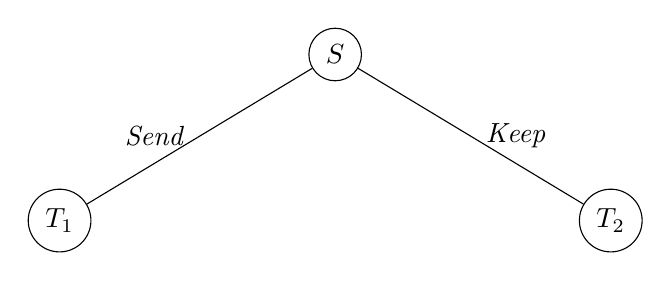
\begin{tikzpicture}[sibling distance=7cm,level distance=6em,every node/.style={shape=circle,align=center}]
          \node[draw]{$S$}
                child[sibling distance = 7cm]{node[draw]{$T_1$} edge from parent node [left] {\emph{Send}}} 
                child[sibling distance = 7cm]{node[draw]{$T_2$} edge from parent node [right] {\emph{Keep}}};
    \end{tikzpicture}
    \centering
    \caption{Two Side Collateral: Both parties report simultaneously}
\end{figure}


\begin{table}[htb!]
    \centering
    \begin{tabular}{ c||c|c| }
        $T_1$& 0$_B$ & 1$_B$   \\
        \hline
        \hline
        0$_S$ & $-U_S(G) | U_B(G)$ & $-U_S(G) - C_S | U_B(G) -  P - C_B$ \\
        \hline
        1$_S$ & $-U_S(G) - C_S | U_B(G) - P - C_B$& $P - U_S(G) | U_B(G) - P$\\ 
        \hline
    \end{tabular}
    \caption{Subgame T1: Both parties report simultaneously}
\end{table}

The subgame $T_1$ has two Nash Equilibria: $\{0_B, 0_S\}$ and $\{1_B, 1_S\}$.\newline
The payout of $\{0_B, 0_S\}$ is $-U_S(G)|U_B(G)$. The payout of $\{1_B, 1_S\}$ is $P-U_S(G)|U_B(G)-P$.
\begin{table}[htb!]
    \centering
        \begin{tabular}{ c||c|c| }
        $T_2$& 0$_B$ & 1$_B$   \\
        \hline
        \hline
        0$_S$ & $0 | 0$ & $-C_S|-P-C_B$ \\
        \hline
        1$_S$ & $-C_S|-P-C_B$ & $P | -P$\\ 
        \hline
    \end{tabular}
    \caption{Subgame T2: Both parties report simultaneously}
\end{table}


The subgame $T_2$ has the same two Nash Equilibria as well: $\{0_B, 0_S\}$ and $\{1_B, 1_S\}$.\newline
The payout of $\{0_B, 0_S\}$ is $0|0$. The payout of $\{1_B, 1_S\}$ is $P|-P$.\newline

The Seller decides if he wants to enter subgame $T_1$ or $T_2$. To analyse his decision we look at his payout from each subgame:\newline
\begin{enumerate}
    \item $T_1$
        \begin{itemize}
            \item $\{0_B, 0_S\}: -U_S(G)$
            \item $\{1_B, 1_S\}: P-U_S(G)$
        \end{itemize}
    \item $T_2$
        \begin{itemize}
            \item $\{0_B, 0_S\}: 0$
            \item $\{1_B, 1_S\}: P$
        \end{itemize}
\end{enumerate}
If we compare these 4 possible payouts:
\[P > P-U_S(G) > 0 > -U_S(G)\]
Without any additional assumptions, it is unclear which is the better subgame for the Seller. He can not choose which subgame is beneficial for him. \newline
We have created a situation where the players do not have all the information they need to choose the best option. That also means, that they are not motivated to behave honestly as they do not know if this is indeed the most beneficial behaviour. As the players are not motivated to behave honestly, they would not trade successfully in this protocol.

\section{An extra input is needed}
The Smart Contract plays an important role in the two side collateral protocol. We want to create a Smart Contract that rewards honest behaviour and punishes dishonest behaviour.\newline 
Problems arise, because the Smart Contract does not know if the physical good $G$ was actually sent to the Buyer. Because of this missing information, it is impossible for the Smart Contract to settle disputes.
\subsection{Ideal Functionality}
We can achieve the ideal functionality of our Smart Contract by giving it the
information whether the good was actually shipped as an input. This ideal functionality is unrealizable without some trusted party that always reports truthfully to the SC. We model the ideal behaviour with a function taking 6 inputs and giving 2 outputs.\newline

\begin{figure}[htbp!]
    \centering
\begin{lstlisting}[language=java]
function assign_coins_ideal(
  buyerCol: natural, sellerCol: natural, price: natural,
  sellerSent: bool /* self reported */, buyerRecv: bool /* self reported */, 
  shipped: bool /* ground truth */
) -> (int /* seller coins */, int /* buyer coins */) {
  if sellerSent == buyerRecv { /* honest case, multiple possible solutions  */ }
  if (not sellerSent) and buyerRecv { /* irrational case, multiple possible solutions */ }

  // both claim they went through and the other player failed
  if shipped {
    sellerCoins: int >= price + sellerCol // honest Seller
    buyerCoins: int < price + buyerCol - U_B(G) // lying Buyer
  } else {
    sellerCoins: int < sellerCol // lying Seller
    buyerCoins: int > price + buyerCol // honest Buyer
  }
  return (sellerCoins, buyerCoins)
}
\end{lstlisting}
\label{fig:code_ideal_sc}
    \caption{General Code for the ideal functionality}
\end{figure}
The irrational case (line 7) should never appear in the real world. At least one player is lying and thereby risking his collateral. Either the Seller did send $G$ but reports that he did not, or B did not receive $G$ but reports that he did. Both behaviours are irrational as the lie would harm the lying party. The irrational case can be implemented without looking at the ground truth. The same can be said about the honest case, as there is no dispute to settle.\newline

The important case is when the seller reports that he shipped the good and the Buyer reports that he did not receive it. Because the Smart Contract has the input 'shipped', it can determine which party is lying and which party is telling the truth.
The Smart Contract settles the disputes in such a way that the honest party has a payout greater than zero and the lying party has a payout smaller than zero. Therefore it is unfavorable for any party to report wrongfully.\newline

We will now see why the function outputs are defined in this way to achieve the ideal functionality:\newline

\minisec{Honest Seller}
The honest Seller (line 11) ships the good to the Buyer and deposits collateral $C_S$. To have a positive payout, his lowest possible return from the smart Contract is $P + C_S$. His payout is at least
\[P + C_S - C_S - U_S(G) = P - U_S(G) > 0\]

\minisec{Lying Buyer}
The Lying Buyer (line 12) receives $G$ and deposits collateral $C_S$ and Price $P$ to the Smart Contract. To have a negative payout, his return from the smart Contract has to be less than $P + Col_B - U_B(G)$. His payout is less than
\[P + C_B - U_B(G) + U_B(G) - C_B -P = 0\]

\minisec{Dishonest Seller}
The dishonest Seller deposits collateral $C_S$ but does not ship the good $G$. To have a negative payout, his return from the smart Contract has to be less than $C_S$. His payout is less than
\[C_S - C_S = 0\]

\minisec{Honest Buyer}
The honest Buyer deposits collateral $C_B$ and Price $P$. To have a positive payout, his return from the smart Contract has to be greater than $P + C_S$. His payout is greater than
\[P + C_S - C_S - P = 0\]

\subsection{Ideal Smart Contract solves the proposed problem}
In the following section we will show that an implementation of the ideal functionality of the Smart Contract indeed creates a game where a successful trade is the Nash Equilibrium. We first write an easy implementation of the ideal SC and then determine the Nash Equilibrium of the created game.
\subsubsection{Implementation of ideal Smart Contract}
The easiest implementation of the honest case is to give back their collateral. If the good was actually shipped, the Seller will be awarded coins of amount $P$, otherwise those coins go back to the Buyer.
In the irrational case the SC will not give any coins back.
In the case of a dispute the SC rewards all the coins to the honest party.

\begin{figure}[htb!]
    \centering
\begin{lstlisting}[language=java]
function assign_coins(
  buyerCol: natural, sellerCol: natural, price: natural,
  sellerSent: bool, buyerRecv: bool, shipped: bool
) -> (int /* seller coins */, int /* buyer coins */) {
  if sellerSent == buyerRecv { 
    sellerCoins = sellerCol // give back the collateral
    buyerCoins = buyerCol // give back the collateral
    if shipped{sellerCoins += price} // G was shipped, Seller gets price
    else {buyerCoins += price}// G was not shipped, Buyer gets price
    }
  if (not sellerSent) and buyerRecv { 
    sellerCoins = 0 // irrational case, give both parties no coins
    buyerCoins = 0
  }

  // both claim they went through and the other player failed
  if shipped {
    sellerCoins = price + sellerCol + buyerCol // honest Seller
    buyerCoins =  0 // lying Buyer
  } else {
    sellerCoins = 0 // lying Seller
    buyerCoins = price + sellerCol + buyerCol // honest Buyer
  }
  return (sellerCoins, buyerCoins)
}
\end{lstlisting}
    \caption{Example Code for an implementation of the ideal Smart Contract}
\end{figure}

With this ideal Smart Contract we can create a new game. We can use any two-side collateral protocol of section~\ref{sec:two-side-collateral}. In this example we will let the Seller report first (c.f.~figure~\ref{pro:two-side-collateral-seller-first}).

\begin{figure}[htb!]
    \centering
\begin{tikzpicture}[sibling distance=7cm,level distance=6em,every node/.style={shape=circle,align=center}]
    \node[draw]{$S$}
        child[sibling distance = 9cm]{node[draw]{$S$}
    		child[sibling distance = 5cm]{node[draw]{$B$}
    		    child[sibling distance = 3cm]{node{1} edge from parent node [left] {0}}
    		    child[sibling distance = 3cm]{node{2} edge from parent node [right] {1}}edge from parent node [left] {0}}
    		child[sibling distance = 5cm]{node[draw]{$B$}
    		    child[sibling distance = 3cm]{node{3} edge from parent node [left] {0}}
    		    child[sibling distance = 3cm]{node{4} edge from parent node [right] {1}}edge from parent node [right] {1}}edge from parent node [left] {\emph{Send}}} 
        child[sibling distance = 9cm]{node[draw]{$S$}
            child[sibling distance = 5cm]{node[draw]{$B$}
                child[sibling distance = 3cm]{node{5} edge from parent node [left] {0}}
    		    child[sibling distance = 3cm]{node{6} edge from parent node [right] {1}}edge from parent node [left] {0}}
            child[sibling distance = 5cm]{node[draw]{$B$}
                child[sibling distance = 3cm]{node{7} edge from parent node [left] {0}}
    		    child[sibling distance = 3cm]{node{8} edge from parent node [right] {1}}edge from parent node [right] {1}}edge from parent node [right] {\emph{Keep}}};
\end{tikzpicture}
    \caption{Payout with an ideal Smart Contract}
    \label{fig:payout-ideal-sc}
\end{figure}
\begin{table}[htb!]
    \centering
    \begin{tabular}{ |c|c| }
    \hline
    & Payout  \\
    \hline
    \hline
    1& $-U_S(G) | U_B(G)$\\
    \hline
    2& $-U_S(G) - C_S| U_B(G)-P - C_B  $\\
    \hline
    3&$P-U_S(G) + C_B | U_B(G)-P - C_B$ \\
    \hline
    4& $P-U_S(G)| U_B(G)-P$\\
    \hline
    5& $0|0$\\
    \hline 
    6& $P + C_B |-P - C_B$\\
    \hline
    7& $- C_S| C_S$\\
    \hline
    8& $P| -P$\\
    \hline
    \end{tabular}
    \caption{The corresponding payout table of figure \ref{fig:payout-ideal-sc}}
\end{table}

Remark: If any party does not send the collateral, the Smart Contract will release the collateral of the the other party and it would result in a payout of $0|0$. This option is not analyzed in the Game tree but has to be considered as an option for each party.\newline

We again start at the bottom of the tree at the Buyer's decision. A rational Buyer would choose: 
\begin{itemize}
    \item 1 over 2 ($U_B(G) > U_B(G) - P - C_B$)
    \item 4 over 3 ($U_B(G) - P > U_B(G) - P - C_B $)
    \item 5 over 6 ($0> -P-C_B$)
    \item 7 over 8 ($C_S > -P$)
\end{itemize}
Out of these options the Seller would choose outcome 4 (\emph{Send},$1$), as this is the best outcome for him.
The Nash Equilibrium is at \{\emph{Send}, 1, 1\} and the trade would unravel successfully.\newline

Such a smart contract solves the problem completely as the Nash Equilibrium lies in both parties behaving honestly.
%TODO It resembles the case of shipping a digital verifiable good. %quote the paper that solved this problem
\subsection{Real World Functionality}
In the real world, the Smart Contract does not know the ground truth. Therefore the signature of a function realizable in the real world is:\newline
\begin{figure}[htb!]
\begin{lstlisting}[language=java]
function assign_coins_real(
  buyerCol: natural, sellerCol: natural, price: natural,
  sellerSent: bool, buyerRecv: bool
) -> (int /* seller coins */, int /* buyer coins */)
\end{lstlisting}
 \centering
    \caption{Signature of a function realizable in the real world}
    \label{fig:real_world_function_signature}
\end{figure}

This poses the following problem: The ground truth is needed to settle disputes. Even if all the other inputs are the same, the output of the ideal functionality depends on the last input. Without this input, previously different scenarios become indistinguishable for the Smart Contract. In the following section we will show that no real world function(a function that does not have the ground truth as input) can achieve the ideal functionality.\newline

Notation: $C_S$: Seller collateral, $C_B$: Buyer collateral, $P$ price, $R_S$ boolean value reported by the Seller, $R_B$: boolean value reported by the Buyer, $S$: ground truth if good was shipped

\paragraph{Theorem:}There is no function $assign\_coins\_real: (C_B, C_S, P, S_B, B_S) \to (O_S, O_B)$ \niknote{maybe $\mathbb{N}\times \mathbb{N}\times \mathbb{N}\times \{0,1\}\times \{0,1\}\times \{0,1\} \to \mathbb{R}\times \mathbb{R}$ is formally more correct, but more difficult for the reader as they do not see what the inputs correspond to}, such that
 $\forall C_B, C_S, P\in \mathbb{N}, \forall R_B,R_S,S \in \{0,1\}$:
\begin{equation}
\label{eq:theorem}
    assign\_coins\_real(C_B, C_S, P, S_B, B_S) = assign\_coins\_ideal(C_B, C_S, P, S_B, B_S,S)
\end{equation}

whereas "$=$" denotes that the output of $assign\_coins\_real$ is in the range defined by the ideal functionality.\newline
\paragraph{Proof:}\label{sec:proof} 
We provide a proof by contradiction: Let us assume for the sake of contradiction that the Theorem is wrong. That means there exists a \niknote{deterministic?} function $assign\_coins\_real : (C_B, C_S, P, S_B, B_S) \to (O_S, O_B)$, such that $\forall C_B, C_S, P\in \mathbb{N}, \forall R_B,R_S,S \in \{0,1\}$ equation \ref{eq:theorem} holds.\newline

We provide the following set of inputs: $C_B=5,C_S=5,P=4,R_S=1,R_B=0,S=1$.
\niknote{I can also put the generic terms $C_S, C_B...$ here instead of concrete numbers}By definition of the ideal functionality (c.f. figure~\ref{fig:code_ideal_sc}), its payoff to the Seller(the first value of the output tuple) has to be:
\begin{equation}
\label{eq:ideal_1}
     assign\_coins\_ideal(C_S=5,C_B=5,P=4,R_S=1,R_B=0,S=1)[1] \geq  5 + 4 = 9
\end{equation}

From equation \ref{eq:theorem} and equation \ref{eq:ideal_1} we get:
\begin{equation}
\label{eq:real_1}
     assign\_coins\_real(C_S=5,C_B=5,P=4,R_S=1,R_B=0)[1] \geq 9
\end{equation}

We now change the last sixth input from 1 to 0: $C_B=5,C_S=5,P=4,R_S=1,R_B=0,S=0$. The payoff from the ideal function(c.f. figure~\ref{fig:code_ideal_sc}) to the Seller has to be:
\begin{equation}
\label{eq:ideal_2}
    assign\_coins\_ideal(C_S=5,C_B=5,P=4,R_S=1,R_B=0,S=0)[1] \leq  4
\end{equation}

From equation \ref{eq:theorem} and equation \ref{eq:ideal_2} we get:
\begin{equation}
\label{eq:real_2}
    assign\_coins\_real(C_S=5,C_B=5,P=4,R_S=1,R_B=0)[1] \leq  4
\end{equation}

As \emph{assign\_coins\_real} is a deterministic function, equation~\ref{eq:real_1} and equation~\ref{eq:real_2} contradict each other. That means that our assumption was wrong and there can not exist such function \emph{assign\_coins\_real}.


%Notation:$sellercol$ is $C_S$...
%%For example, it is impossible to differentiate between a lying seller that did not send the good $G$ but says he did, and a lying Buyer that received the good but says he did not. 
%Without the sixth input, it is impossible to design a Smart Contract that achieves the ideal functionality described in section 5.4.1.
\orfnote{do not hardcode section numbers, use labels/references instead}
\orfnote{I would really like to present this argument in a theorem-proof format}

\chapter{A redesigned game}
As we have shown (c.f.~\ref{sec:formal-proof}) \orfnote{we have to discuss what will be the fate of the
proof}, it is not possible (under our assumptions) to design a protocol that would create a successful game (as described in \ref{sec:the-game}). The biggest problem is that we have no reliable way of telling the Smart Contract whether the physical good $G$ was actually shipped or not. If there is a dispute, the Smart Contract does not know which party is lying and has to be punished.\newline

We need to rework our assumptions and requirements for the game we want to design. For that it is is interesting to see that the two side collateral protocol (c.f.~\ref{sec:two-side-collateral}) is very close to achieving our goals. As already discussed, the problem is that the Seller is not actually incentivized to send the physical good $G$, because the Buyer is not incentivized to report his dishonest behaviour. The Buyer gets a bigger Payout when he lies to the Smart Contract instead of reporting the dishonest behaviour. Therefore a rational Buyer would never punish a dishonest Seller in this scenario. If a Seller thinks that the Buyer would punish him (the Buyer is not acting rational in this scenario), then the Seller is incentivized to send the physical good $G$.\newline
\section{Two Side Collateral with truthful Buyer} 
In this section we show that if the Buyer behaves truthful (and therefore not rationally), it is not beneficial for the Seller to behave dishonestly. The created game would have a successful trade as Nash Equilibrium.\newline
\begin{figure}[htb!]
    \centering
    \begin{tikzpicture}[sibling distance=7cm,level distance=6em,every node/.style={shape=circle,align=center}]
    \node[draw]{$S$}
        child[sibling distance = 8cm]{node[draw]{$S$}
    		child[sibling distance = 4cm]{node[draw]{$B$}
    		    child[sibling distance = 3cm]{node{1} edge from parent node [left] {0}}
    		    child[sibling distance = 3cm]{node{2} edge from parent node [right] {1}}edge from parent node [left] {0}}
    		child[sibling distance = 4cm]{node[draw]{$B$}
    		    child[sibling distance = 3cm]{node{3} edge from parent node [left] {0}}
    		    child[sibling distance = 3cm]{node{4} edge from parent node [right] {1}}edge from parent node [right] {1}}edge from parent node [left] {\emph{Send}}} 
        child[sibling distance = 8cm]{node[draw]{$S$}
            child[sibling distance = 4cm]{node[draw]{$B$}
                child[sibling distance= 3cm]{node{5} edge from parent node [left] {0}}
    		    child[sibling distance = 3cm]{node{6} edge from parent node [right] {1}}edge from parent node [left] {0}}
            child[sibling distance = 4cm]{node[draw]{$B$}
                child[sibling distance = 3cm]{node{7} edge from parent node [left] {0}}
    		    child[sibling distance = 3cm]{node{8} edge from parent node [right] {1}}edge from parent node [right] {1}}edge from parent node [right] {\emph{Keep}}};
    \end{tikzpicture}
    \label{fig:payout-truthful-buyer}
    \caption{Two Side Collateral with truthful Buyer}
\end{figure}

\begin{center}
\begin{tabular}{ |c|c| }
\hline
& Payout  \\
\hline
\hline
1& $-U_S(G) | U_B(G)$\\
\hline
2& $-U_S(G) - C_S| U_B(G)- P - C_B $\\
\hline
3&$P-U_S(G) - C_S | U_B(G) -P - C_B$ \\
\hline
4& $P-U_S(G)| U_B(G)-P$\\
\hline
5& $0|0$\\
\hline 
6& $-C_S |-P - C_B$\\
\hline
7& $- C_S| -P-C_B$\\
\hline
8& $P| -P$\\
\hline
\end{tabular}
\end{center}
\captionof{table}{The corresponding payout table of figure \ref{fig:payout-truthful-buyer}}
Now a truthful Buyer stops acting rationally and chooses option 7 over 8.\newline
The Buyer chooses:
\begin{itemize}
    \item 1 over 2 ($U_B(G) > U_B(G) -P -C_B$)
    \item 4 over 3 ($U_B(G) - P > U_B(G) -P -C_B$)
    \item 5 over 6 ($0 > -P -C_B$)
    \item 7 over 8 (irrational decision)
\end{itemize}
The Seller would choose option 4:
\[P-U_S(G)>0>-U_S(G)>-C_S\]
The Seller now sends the good, because he the Buyer will punish him if he does not send it.
The Nash Equilibrium would be the honest case and the trade would unravel successfully.\newline

At first glance this seems counterintuitive: If the act of reporting benefits the Buyer, why would the rational Buyer not report the misbehaviour of the Seller? As the definition of a rational behaviour is maximizing the own Utility, would it not be rational to report the Seller?
The answer to this question is no. If the Seller has already misbehaved, it is more profitable for the Buyer to not report the misbehaviour, as he at least receives back his collateral.
It is not the act of reporting that is profitable for the Buyer, rather it is
the threat of reporting. This thread has to be considered by the Seller before he chooses whether to misbehave. If the Seller thinks that maybe the Buyer will report him, he is discouraged of trying to cheat and not sending $G$.\newline

The problem lies in the way we laid the rules for the game: As we defined both players as always behaving rationally, the Seller knows that the Buyer can not report him, because it is not the rational decision.
If the Seller did not know that the Buyer is always acting rational, he would be taking a great risk by not sending the physical good: the risk of being exposed and losing his collateral and his money $P$.
We want to create a situation where the Seller evaluates the situation as being too risky to cheat. In this situation the rational Seller will behave honestly and  send $G$.
To conclude: It is sufficient to turn the non credible threat of the Buyer (reporting 0 if $G$ is not shipped) into a credible threat for the double collateral protocol to succeed.\newline

We redesign the game by adding another Entity. Its purpose is to assist the Buyer in convincing the Seller that he will be punished if he does not send $G$. It turns the non credible threat of the Seller's misbehaviour being reported into a credible threat. We need this Entity to maintain the rationality of the Buyer, as a rational Buyer will not report any misbehaviour of the Seller.
If this is achieved, a Seller knows that it is unprofitable to not send $G$.\newline


\section{Formal definition of the new Entity}
\niknote{Maybe change title to "formally redesigning the game"}
We introduce another entity, which we call Mediator $M$: and has the following behaviour:
\begin{definition}[Mediator]
\label{def:mediator}
An Entity $M$ that has the purpose to protect the Buyer from an misbehaving Seller. $M$ has the following behaviour:
\begin{enumerate}
    \item receive SC address and specifications that describe $G$
    \item receive the physical good
    \item check if the the physical good match the description for $G$
    \begin{itemize}
        \item if so: report 1 to the SC and send the good to the Buyer
        \item else: destroy the good and report 0 to the SC
    \end{itemize}
\end{enumerate}
\end{definition}

The new Entity is not modeled as a rational party. It always behaves in the described way. It has its own physical address and the power to receive physical items. Given the right specifications of $G$, the Mediator can distinguish $G$ from every other  physical item. The Mediator also has the power to communicate with the Smart Contract and the Buyer. It is trusted by the Buyer to evaluate if the good sent by the Seller is indeed $G$.
//TODO Maybe expand on that: What about trust
\section{Mediated protocol}
\label{sec:mediated-protocol}
We propose the following protocol:
\begin{figure}[htb!]
\fbox{
 \procedureblock[linenumbering]{Mediated protocol}{
    \text{Buyer gives SC address and specifications for $G$ to the Mediator}\\
    \text{Seller deposits collateral $C_S > P$ to the Smart Contract}\\
    \text{Buyer deposits collateral $C_B > P$ and price $P$ to the Smart Contract}\\
    \text{Seller sends physical good $G$ to the Mediator and reports it to the Smart Contract}\\
    \text{Mediator receives the physical good, confirms it to the Smart Contract and sends $G$ to the Buyer}\\
    \text{The Smart Contract releases the collateral of the Seller and the Buyer and sends $P$ to the seller}
}
}
    \centering
    \caption{Mediated protocol description}
    \label{pro:mediated-protocol}
\end{figure}

\begin{figure}[htb!]
\procedureblock{Mediated Protocol}{
\textbf{$S$} \<\< \textbf{SC} \<\<  \textbf{M} \<\< \textbf{$B$} \\
%------------TELL THE MEDIATOR---------------
\< \< \< \< \sendmessageleft{top=information,length=2cm} \>\>\pclb
%-----------COLLATERAL-----------------
\pcintertext [dotted] {Deposit Collateral} \\
\< \sendmessageright{top = $C_S$,length=2cm} \< \<  \sendmessageleftx[5.5cm]{4}{C_B} \<   \pclb
\pcintertext [dotted] {Send Resources} \\
%-----------SEND P------------------
\< \< \< \sendmessageleftx[5.5cm]{8}{P} \< \< \< \\
%-----------SEND G------------------------
\< \sendmessagerightx[6cm]{6}{G} \<\< \pclb
\pcintertext [dotted] {Report to the SC} \\
%-----------SELLER REPORTS----------------------
\< \sendmessageright{top=report 1,length=2cm} \< \< \< \< \< \\
%---------------CHECK IF G IS RIGHT-------------
\< \< \< \< \text{$G$ is right?} \< \< \\
%-----------MEDIATOR REPORTS---------------
\< \< \< \sendmessageleft{top=report 1,length=2cm} \< \< \< \\
%------MEDIATOR SENDS G TO $B$-------------
\< \< \< \< \sendmessageright{top=$G$,length=2cm} \>\>\pclb
\pcintertext [dotted] {Pay back collateral} \\
\<  \sendmessageleft{top=$C_S$,length=2cm} \<\<\<\<\< \\
\< \< \< \sendmessagerightx[5.5cm]{8}{C_B} \< \< \< \\
}
    \centering
    \caption{Mediated Protocol}
    \label{fig:mediated-protocol}
\end{figure}
\subsection{Honest behaviour}
\niknote{Maybe honest behaviour as well with Cryptocode}
This new protocol does change the honest behaviour of the Buyer. His honest behaviour is now:
\begin{enumerate}
    \item Tell the right SC address and the right specifications for $G$ to the Mediator
    \item Deposit $C_B>P$ to the Smart Contract
    \item Send funds of amount $P$ to the Smart Contract
    \item Wait and receive $G$ from the Mediator
\end{enumerate}
It is important that the Buyer no longer reports to the Smart Contract, as this responsibility is handed over to the Mediator.\newline
The honest behaviour of the Seller remains unchanged by the new protocol. It still is:
\begin{enumerate}
    \item Deposit $C_S>P$ to the Smart Contract
    \item Send $G$ to the provided address (which is now the Mediator's)
    \item Report to the Smart Contract  that $G$ was sent
\end{enumerate}

\subsection{Possible Strategies}
The new protocol has no impact on the possible strategies for the Seller. He still has the option to either send (\emph{Send}) or keep (\emph{Keep}) the physical good. After that, he has the option to report 0 or 1 to the Smart Contract.
As the Buyer does not longer report to the Smart Contract, he has fewer decisions to make. As soon as he enters the trade (pays the collateral and $P$ to the SC), he no longer has any decision to make. The Mediator will take care of reporting to the Smart Contract.

We again start our analysis at point 4 of the protocol.\newline

\begin{figure}[htb!]
    \centering
    \begin{tikzpicture}[sibling distance=7cm,level distance=6em,every node/.style={shape=circle,align=center}]
    \node[draw]{$S$}
        child[sibling distance = 8cm]{node[draw]{$S$}
    		child[sibling distance = 5.5cm]{node[draw]{M}
    		    child[sibling distance = 5cm]{node[shape = rectangle]{$-U_S(G) - C_S| - P - C_B $} edge from parent node [right] {1}}edge from parent node [left] {0}}
    		child[sibling distance = 5.5cm]{node[draw]{M}
    		    child[sibling distance = 3cm]{node[shape = rectangle]{$P-U_S(G)| U_B(G)-P$} edge from parent node [right] {1}}edge from parent node [right] {1}}edge from parent node [left] {\emph{Send}}} 
        child[sibling distance = 8cm]{node[draw]{$S$}
            child[sibling distance = 4cm]{node[draw]{M}
    		    child[sibling distance = 3cm]{node[shape = rectangle]{$0|0$} edge from parent node [right] {0}}edge from parent node [left] {0}}
            child[sibling distance = 4cm]{node[draw]{M}
    		    child[sibling distance = 3cm]{node[shape = rectangle]{$- C_S| -P-C_B$} edge from parent node [right] {0}}edge from parent node [right] {1}}edge from parent node [right] {\emph{Keep}}};
    \end{tikzpicture}
    \caption{Two Side Collateral with ideal Mediator}
\end{figure}

\orfnote{Why does $S$ report before $M$? Discuss. Mention that, at the end of
the day, since this game works and we achieved our goal, we don't really care
about small differences like this.}
\niknote{maybe here complete tree as it is our final solution?}
The Seller can choose the one option which yields him the biggest payout. This is sending the good (\emph{Send}) and reporting 1, as: 

\[P-U_S(G)>0>-C_S>-U_S(G) - C_S\]

It is the best option for the Seller to successfully trade with the Buyer.
The Buyer would also engage in the trade, because it is profitable for him:
\begin{itemize}
    \item $U_B(G) -P > 0$
\end{itemize}
The Nash Equilibrium of this game is both players trading successfully. This game achieves the goal formulated in section~\ref{sec:goal}.

\section{Possible realizations of Mediator}
The Mediator, as it is defined in 6.1, is a theoretical Entity. In the following section we will discuss some practical attempts to realize the Mediator.
\subsection{Friend of Buyer reports}
As the Buyer has to trust the Mediator, one possible approach is choosing a loyal friend of the Buyer to be the Mediator. It is important that he is loyal to the Buyer, meaning that he will not betray the Buyer and keep the physical good $G$ to himself. The Buyer fully trusts his loyal friend.\newline

The friend will not act rational, as he does not want to maximize his own Utility. He rather wants to maximize the Buyer's utility. Therefore he will always choose the option that maximizes the payout of the Buyer.
The Friend($F$) will receive the physical good $G$ and check if it matches the agreed good. After that, he reports 0 (received the good successfully) or 1 (did not receive the good successfully) to the Smart Contract. After that he will send the $G$ to the Buyer.\newline

\begin{figure}[htb!]
\fbox{
 \procedureblock[linenumbering]{Two side collateral: Friend reports}{
    \text{Seller deposits collateral $C_S > P$ to the Smart Contract}\\
    \text{Buyer deposits collateral $C_B > P$ and price $P$ to the Smart Contract}\\
    \text{Seller sends physical good $G$ to the Friend of the Buyer and reports it to the Smart Contract}\\
    \text{Friend of the Buyer receives the physical good and reports it to the Smart Contract}\\
    \text{The Smart Contract releases the collateral of the Seller and the Buyer and sends $P$ to the Seller}\\
    \text{Friend sends $G$ to the Buyer}
}
}
    \centering
    \caption{Two side collateral protocol: Friend of Buyer reports}
    \label{pro:two-side-collateral-friend}
\end{figure}

To increase readability, we do not plot the decisions from point 1 and point 2.
If someone does not deposit the collateral, the Smart Contract aborts the trade
and the payout is $0|0$.\newline

\begin{tikzpicture}[sibling distance=7cm,level distance=6em,every node/.style={shape=circle,align=center}]
    \node[draw]{$S$}
        child[sibling distance = 8cm]{node[draw]{$S$}
    		child[sibling distance = 4cm]{node[draw]{F}
    		    child[sibling distance = 3cm]{node{1} edge from parent node [left] {0}}
    		    child[sibling distance = 3cm]{node{2} edge from parent node [right] {1}}edge from parent node [left] {0}}
    		child[sibling distance = 4cm]{node[draw]{F}
    		    child[sibling distance = 3cm]{node{3} edge from parent node [left] {0}}
    		    child[sibling distance = 3cm]{node{4} edge from parent node [right] {1}}edge from parent node [right] {1}}edge from parent node [left] {\emph{Send}}} 
        child[sibling distance = 8cm]{node[draw]{$S$}
            child[sibling distance = 4cm]{node[draw]{F}
                child[sibling distance = 3cm]{node{5} edge from parent node [left] {0}}
    		    child[sibling distance = 3cm]{node{6} edge from parent node [right] {1}}edge from parent node [left] {0}}
            child[sibling distance = 4cm]{node[draw]{F}
                child[sibling distance = 3cm]{node{7} edge from parent node [left] {0}}
    		    child[sibling distance = 3cm]{node{8} edge from parent node [right] {1}}edge from parent node [right] {1}}edge from parent node [right] {\emph{Keep}}};
\end{tikzpicture}

\begin{center}
\begin{tabular}{ |c|c| }
\hline
& Payout  \\
\hline
\hline
1& $-U_S(G) | U_B(G)$\\
\hline
2& $-U_S(G) - C_S| U_B(G)- P - C_B $\\
\hline
3&$P-U_S(G) - C_S | U_B(G) -P - C_B$ \\
\hline
4& $P-U_S(G)| U_B(G)-P$\\
\hline
5& $0|0$\\
\hline 
6& $-C_S |-P - C_B$\\
\hline
7& $- C_S| -P-C_S$\\
\hline
8& $P| -P$\\
\hline
\end{tabular}
\end{center}

We again start at the bottom of the tree to analyze the payout. As F wants to maximize the payout of the Buyer, he will choose:
\begin{itemize}
    \item 1 over 2 ($U_B(G) > U_B(G) -P -C_B$)
    \item 4 over 3 ($U_B(G) - P > U_B(G) -P -C_B$)
    \item 5 over 6 ($0 > -P -C_B$)
    \item 8 over 7 ($-P > -P -C_B)$)
\end{itemize}
The Seller would choose option 8, as 
\[P>P-U_S(G)>0>-U_S(G)\]
Because the payout of the Buyer is $-P<0$, he would not engage in this trade and therefore refuse to pay the collateral in step 1. The trade is still unsuccessful.\newline

We modeled the friend as being loyal to the Buyer. He wants to maximize the utility of the Buyer.
That means that he will always choose the behaviour that benefits the Buyer. In the case where the Seller does not send $G$ but lies to the SC and reports 1, the friend of the Buyer will also report 1. In this crucial case he will behave exactly like the Buyer. That means that the game does not change for the Seller. It is still profitable for him to deviate from the protocol and not send $G$.\newline

The friend is not suited as being the Mediator. He does not achieve the same functionality as the ideal Mediator proposed in definition~\ref{def:mediator}, as he will not always report truthfully to the Smart Contract. As the Seller knows this, he can take advantage of it. He knows that he will not be punished if he does not send the physical good. The friend as Mediator is not a credible threat to the Seller, as he will report exactly like the Buyer would. Therefore a rational Seller will not send the good and this protocol does not achieve the goal proposed in section~\ref{sec:goal}.\newline

Introducing a friend as the Mediator does not solve the problem. The tree and
the payout are exactly the same as in the two-sided collateral protocol (c.f.~\ref{fig:two-side-collateral}).
To solve the problem we need to come up with a Mediator that is fully trusted by
the Buyer, but is not trying to maximize the Buyer's payout.
Every entity that maximizing the payout for the Buyer will not be a
credible threat to the Seller.


\subsection{Postal Office reports}
In our formal analysis we assumed that there is a way for the physical item $G$ to be reliably shipped. In practice physical goods are usually shipped by a another party (Post office/shipping company).
Therefore the parties have to trust the Postal Office (PO) to actually deliver the good. Because the parties already trust the PO, the PO can also report to the Smart Contract and thereby act as the Mediator.\newline

We propose the following protocol:
\begin{figure}[htb!]
\fbox{
 \procedureblock[linenumbering]{Two side collateral: Postal Office as Mediator}{
 \text{Buyer gives SC address and specifications for $G$ to the Postal Office}\\
    \text{Seller deposits collateral $C_S > P$ to the Smart Contract}\\
    \text{Buyer deposits collateral $C_B > P$ and price $P$ to the Smart Contract}\\
    \text{Seller sends physical good $G$ to the Postal Office and reports it to the Smart Contract}\\
    \text{Postal Office receives the physical good and reports it to the Smart Contract}\\
    \text{The Smart Contract releases the collateral of the Seller and the Buyer and sends $P$ to the Seller}\\
    \text{Postal Office sends $G$ to the Buyer}
}
}
    \centering
    \caption{Two side collateral protocol: Postal Office as Mediator}
    \label{pro:two-side-collateral-postal}
\end{figure}

\subsubsection{Postal Office realises ideal Mediator}
An honest Postal Office realises the ideal Mediator as defined in 6.1:
\begin{enumerate}
    \item It receives the SC address and specifications that describe G
    \item It receives the physical good from the Seller
    \item It checks, if the received good matches the specifications for $G$
        \begin{itemize}
            \item if so, it reports 1 and sends the good to the Buyer
            \item else it reports 0 and destroys the good
        \end{itemize}
\end{enumerate}
As the Postal Office has to be trusted by the Buyer, it meets the requirements to being the ideal mediator. We have already shown (6.2) that a practical implementation of the ideal Mediator would solve our problem. Therefore the Postal Office reporting to the Smart Contract and thereby acting as Mediator is a viable solution to the problem.
\minisec{Trust in the Postal Office}
Although this solution with the PO as Mediator achieves an incoercible sale of the physical good $G$, both parties still have to trust the Postal Office behave honestly.
In addition to that, the Postal Office now knows the specifications of the good being shipped. This means that there is less privacy for the Buyer and the Seller. If the physical good that is being shipped is very valuable, it opens up possible attacks by the Postal Office.\newline

-po has to be big/trusted enough\newline
-exit scams?
\minisec{Difference Postal Office and Escrow}
The big difference between the Postal Office and traditional third party escrow is that the PO does not handle the money. 
In traditional third party escrows, the escrow has to be trusted with the good and the money. As it is in possession of both, it opens up possibilities to scam the Buyer and the Seller out of both the money and the physical good.
As the postal Office is only holding on to the physical good, the reward of a
possible scam is considerably less than if it also had control of the money (approximately half, assuming that $U_{PO}(G) \approx P$). \newline 

We trust the PO by default? Third party escrow is third rational party therefore can scam, but PO is not modeled as rational party? kind of cheating
\subsection{Machine reports}
If we can build a machine that can recognize $G$ reliably, we can completely eliminate trust. This machine can act as the Mediator. It does not make decisions, it simply takes inputs and acts accordingly.\newline
The inputs it takes are:
\begin{itemize}
    \item The address of the SC
    \item Specifications that describe $G$
    \item The physical good $G$
\end{itemize}

The Mediator now is a deterministic machine in contrast to a third Entity. This has the advantage that both the Buyer and the Seller know that the Machine will behave exactly as it is programmed to do. It can presumably can use some kind of image recognition or 3D object recognition. \niknote{find references}. This machine has to be cheap
and open source, therefore both parties can verify its code and the Seller can
easily believe that the Buyer can have such a machine, thus eliminating trust.

\subsubsection{Behaviour of the Machine}
\begin{enumerate}
    \item It receives the SC address and specifications that describe G
    \item It receives the physical good from the Seller
    \item It checks, if the received good matches the specifications for $G$
        \begin{itemize}
            \item if so: it reports 1 and sends the good to the Buyer
            \item else: it reports 0 and destroys the good
        \end{itemize}
\end{enumerate}
A Machine with this behaviour is realising the ideal Mediator from 6.1. 

\subsubsection{Protocol}
\begin{figure}[htb!]
%\fbox{
 \procedureblock[linenumbering]{Two side collateral: Machine as Mediator}{
 \text{Buyer gives SC address and specifications for $G$ to the Machine}\\
    \text{Seller deposits collateral $C_S > P$ to the Smart Contract}\\
    \text{Buyer deposits collateral $C_B > P$ and price $P$ to the Smart Contract}\\
    \text{Seller sends physical good $G$ to the Machine and reports it to the Smart Contract}\\
    \text{Machine receives the physical good and reports it to the Smart Contract}\\
    \text{The Smart Contract releases the collateral of the Seller and the Buyer and sends $P$ to the Seller}\\
    \text{Machine sends $G$ to the Buyer}
}
%}
    \centering
    \caption{Two side collateral protocol: Machine as Mediator}
    \label{pro:two-side-collateral-machine}
\end{figure}

As the machine realises an ideal ideal Mediator (6.1), this protocol achieves an incoercible sale of $G$.\newline
In addition to that, no trust is needed as the Mediator is not able to behave differently. It will always behave as it was programmed to behave. Therefore it is not able to perform any kind of scam.

\subsubsection{Realizability of the machine} 
The biggest challenge for the machine is to determine if the provided good actually matches the specifications.\newline
We believe that a machine which behaves exactly as we described is could be
realised using artificial intelligence. 
\niknote{maybe merge this paragraph with the one directly above Behaviour of the Machine}\orfnote{expand a bit. Mention image/3d
object recognition. Find references}


\section{Difference from trusted third party/ Escrow}
\niknote{not yet implemented}
How is the reporting entity different than an escrow?
-only buyer has to trust?
-Maybe even model rational: misbehaving is doing more damage to the company/manufacturer than behaving exactly as described -> then no trust is necessary -> but then we can us it as a clean middleman that reports to the SC
%\chapter{Open Research/ Questions}

\chapter{Conclusion}
%what?(short form) \newline
\niknote{still need to add references}\newline
Cryptocurrencies gain acceptance as a valid payment method for digital and physical goods. There is a need for a protocol that handles these sales with a cryptocurrency as payment method. Current solutions use a trusted third party. As there are situations where no trusted third party is available and the third party can misbehave, protocols without the need of that trust are advantageous. The goal of this thesis was to find such a protocol that enables a trustless and incoercible sale of physical goods over a blockchain.\newline

 First, we formalized the problem. After that we proposed two-party protocols and analyzed if these protocols are viable solutions to the formalized problem. First we examined protocols without collateral. Then we looked at protocols where only one party deposits collateral. After showing that these approaches do not solve the proposed problem, we looked at protocols where both parties deposit collateral. As all of these candidates did not solve the proposed problem, we tried to prove that such a two-party protocol is impossible. \niknote{Here write something about the proof} After showing that indeed such a two-party protocol is impossible, we lowered the requirements for the protocol by allowing a Mediator which is trusted by the Buyer. We showed that with this mediator there exists a protocol that enables a trustless and incoercible sale of physical goods. We proposed such a protocol with an idealised Mediator in section \ref{sec:mediated-protocol}. At the end of the thesis, we looked at possible practical realizations that can take the role of the Mediator. We proposed two possible solutions (Postal Office reports, Machine reports).

%How?\newline
%Looked first at no collateral, then.... then... (like intro), but no results\newline
%Then tried to proof that this problem is not solvable unter the first assumptions.\newline
%Then tried to change the problem. (loose up the restrictions) We allowed another entity, M to be apart of the protocol... we showed that with a mediator behaving like ref (ideal mediator) the problem has a solution. We proposed a protocol that solves this problem (ref). We then searched for possible practical realizations of a Mediater and proposed 2 working solutions (PO, Machine) They 

%what are the results of this thesis?

\section{Outlook}
maybe find a formal way to distinguish working protocols from not working ones, given the new assumptions where we allow a Mediator? probably dependend on the behaviour of the Mediator. why is it working? Is there an easier protocoll that still solves the problem?\newline

Engeneer the (ML) machine, as in section... that can classify a physical good correctly with high probability. 
Object detection with 3d model. maybe loook at face ID?


\chapter{test}
\subsection{without subprocedure}
\procedureblock{Protocol with Mediator}{
\textbf{$S$} \<\< \textbf{SC} \<\<  \textbf{M} \<\< \textbf{$B$} \\
%------------TELL THE MEDIATOR---------------
\pcln \< \< \< \< \sendmessageleft{top=information,length=2cm} \>\>\pclb
%-----------COLLATERAL-----------------
\pcintertext [dotted] {Deposit Collateral} \\
\pcln \< \sendmessageright{top = $C_S$,length=2cm} \< \<  \sendmessageleftx[5.5cm]{4}{C_B} \<   \pclb
\pcintertext [dotted] {Send Resources} \\
%-----------SEND P------------------
\pcln \< \< \< \sendmessageleftx[5.5cm]{8}{P} \< \< \< \\
%-----------SEND G------------------------
\pcln  \< \sendmessagerightx[6cm]{6}{G} \<\< \pclb
\pcintertext [dotted] {Report to the SC} \\
%-----------SELLER REPORTS----------------------
\pcln \< \sendmessageright{top=report 1,length=2cm} \< \< \< \< \< \\
%---------------CHECK IF G IS RIGHT-------------
\pcln \< \< \< \< \text{$G$ is right?} \< \< \\
%-----------MEDIATOR REPORTS---------------
\pcln \< \< \< \sendmessageleft{top=report 1,length=2cm} \< \< \< \\
%------MEDIATOR SENDS G TO $B$-------------
\pcln \< \< \< \< \sendmessageright{top=$G$,length=2cm} \>\>\pclb
\pcintertext [dotted] {Pay back collateral} \\
\pcln \<  \sendmessageleft{top=$C_S$,length=2cm} \<\<\<\<\< \\
\pcln \< \< \< \sendmessagerightx[5.5cm]{8}{C_B} \< \< \< \\
}
\subsection{with subprocedure}
\newpage
\procedureblock{Protocol with Mediator}{
\textbf{$S$} \<\< \textbf{SC} \<\<  \textbf{M} \<\< \textbf{$B$} \\
%------------TELL THE MEDIATOR---------------
\pcln \< \< \< \< \sendmessageleft{top=information,length=2cm} \>\>\pclb
%-----------COLLATERAL-----------------
\pcintertext [dotted] {Deposit Collateral} \\
\pcln \< \sendmessageright{top = $C_S$,length=2cm} \< \<  \sendmessageleftx[5.5cm]{4}{C_B} \<   \pclb
\pcintertext [dotted] {Send Resources} \\
%-----------SEND P------------------
\pcln \< \< \< \sendmessageleftx[5.5cm]{8}{P} \< \< \< \\
%-----------SEND G------------------------
\pcln  \< \sendmessagerightx[6cm]{6}{G} \<\< \pclb
\pcintertext [dotted] {Report to the SC} \\
%-----------SELLER REPORTS----------------------
\pcln \< \sendmessageright{top=report 1,length=2cm} \< \< \< \< \< \\
%---------------CHECK IF G IS RIGHT-------------
\pcln \< \< \< \< 
\dbox{ \begin{subprocedure} \pseudocodeblock[linenumbering]{
\pcif \text{G matches instructions}\\
\pcthen \text{report 1 and send $G$ to Buyer} \\
\pcelse \text{report 0 and destroy $G$}
}
\end{subprocedure}}
\< \< \\
%-----------MEDIATOR REPORTS---------------
\pcln \< \< \< \sendmessageleft{top=report ,length=2cm} \< \< \< \\
%------MEDIATOR SENDS G TO $B$-------------
\pcln \< \< \< \< \sendmessageright{top=$G$,length=2cm} \>\>\pclb
\pcintertext [center] {Pay back collateral} \\
\pcln \<  \sendmessageleft{top=$C_S$,length=2cm} \<\<\<\<\< \\[][\hline]
\pcln \< \< \< \sendmessagerightx[5.5cm]{8}{C_B} \< \< \< \\
}

\section{two-Side collateral}
\minisec{How it is now}
\begin{enumerate}
    \item Seller deposits collateral $C_S > P$ to the Smart Contract
    \item Buyer deposits collateral $C_B > P$ to the Smart Contract
    \item Buyer sends funds of amount $P$ \orfnote{sends $P$ coins} to the Smart
    Contract \orfnote{this step could be combined with the previous one}
    \item Seller sends physical good $G$ to the seller and reports it to the Smart Contract
    \item Buyer receives the physical good and confirms \orfnote{reports} it to the Smart Contract
    \item The Smart Contract releases the collateral of the Seller and the Buyer and sends $P$ to the Seller
\end{enumerate}
\minisec{cryptocode figure}
\procedureblock{Two-Side-Collateral Protocol}{
\textbf{$S$} \<\< \textbf{SC} \<\< \textbf{$B$} \pclb
%-----------COLLATERAL-----------------
\pcintertext [dotted] {Deposit Collateral} \\
\pcln \< \sendmessageright{top = $C_S$} \< \<  \sendmessageleft{top = $C_B$} \<   \pclb
\pcintertext [dotted] {Send Resources} \\
%-----------SEND P------------------
\pcln \< \< \< \sendmessageleft{top = $P$} \< \\
%-----------SEND G------------------------
\pcln  \< \sendmessagerightx[6cm]{6}{G} \<\< \pclb
\pcintertext [dotted] {Report to the SC} \\
%-----------SELLER REPORTS----------------------
\pcln \< \sendmessageright{top=report 1} \< \< \< \\
\pcln \< \< \< \sendmessageleft{top = report} \< \text{check, if $G$ correct} \\
\pcln \<  \sendmessageleft{top=$P$} \<\<\< \pclb
%---------------CHECK IF G IS RIGHT-------------
%\pcln \< \< \< \< \text{$G$ is right?} \< \< \\
\pcintertext [dotted] {Pay back collateral} \\
\pcln \<  \sendmessageleft{top=$C_S$} \<\<\< \\
\pcln \< \< \< \sendmessageright{top=$C_B$} \<  \\
}

\minisec{cryptocode proocedure}
\begin{figure}[htb!]
%\fbox{
 \procedureblock[linenumbering]{Protocol}{
    \text{Seller deposits collateral $C_S > P$ to the Smart Contract}\\
    \text{Buyer deposits collateral $C_B > P$ and $P$ coins to the Smart Contract}\\
    \text{Seller sends physical good $G$ to the seller and reports it to the Smart Contract}\\
    \text{Buyer receives the physical good and reports it to the Smart Contract}\\
    \text{The Smart Contract releases the collateral of the Seller and the Buyer and sends $P$ to the Seller}
}
%}

    \centering
    \caption{Double collateral protocol}
    \label{pro:double-collateral-protocol}
\end{figure}

 %\begin{figure}[!htbp]
    %\begin{systembox}{A}
%	ss
    %\end{systembox}
 %\end{figure}
	
	%\bibliographystyle{}
	
	%\bibliography{references.bib}
	\printbibliography
	
	\appendix

\end{document}
